%!TEX root = ../template.tex
%%%%%%%%%%%%%%%%%%%%%%%%%%%%%%%%%%%%%%%%%%%%%%%%%%%%%%%%%%%%%%%%%%%%
%% chapter5.tex
%% NOVA thesis document file
%%
%% Chapter with lots of dummy text
%%%%%%%%%%%%%%%%%%%%%%%%%%%%%%%%%%%%%%%%%%%%%%%%%%%%%%%%%%%%%%%%%%%%

\typeout{NT FILE chapter5.tex}%

\iffalse
\newcommand{\property}[2]{%
  \begin{center}
    \begin{tabular}{@{}>{\itshape}l@{\hspace{1em}}l@{}}
      #1 & \textbf{(P\textsubscript{#2})}
    \end{tabular}
  \end{center}
}
\fi

\usetikzlibrary{arrows.meta, positioning, automata, shapes.geometric}

\RecustomVerbatimEnvironment{Verbatim}{BVerbatim}{} % to center minted

\chapter{WALTZ}
\label{cha:waltz}
In this chapter, we introduce WALTZ \fl \musQuarter, the specification language that allows us
to specify the relations between actor interactions, the messages that they
exchange, and relate the contents of the messages exchanged in the system.
Notably, the language semantics allow for context-aware verification of
properties, which is one of its main strengths in highly concurrent distributed
client-server systems.

WALTZ is designed around three fundamental abstractions that directly
correspond to the concepts of actor-based systems: actors are autonomous
computational entities, message patterns are the communication signatures
between them, and state bindings that will correlate information across chained
interactions of messages. These abstractions work together to provide a natural
and intuitive way to express properties that span multiple actors. Broadly, the
language consists of two key components. One dictates the control flow of the
messages, defining how messages are exchanged, chained, and related across
different actors. The other focuses on verifying logical properties within the
content of these messages, ensuring correctness within the established flow.

\section{Motivation}
\label{sec:waltz_motivation}

The necessity of defining a specification language for actor-based systems
arise from the paradigm these systems follow and the limitations of other
formalisms and tools in addressing such systems. The differences are explained
in more detail in \Cref{cha:related_work}.

\iffalse
\texttt{detectEr}~\cite{attard2017runtime},
specification language used does not allow to express properties that span
across multiple actor communication, and co-relate those messages. Even if the
language itself allows such, the fragment that is used by the tool only allows
for the monitoring of a single process. On top of that, using \texttt{detectEr}s formalism
we must specify all the possible interleavings of the messages due to the
concurrency model of \texttt{Erlang}, which is cumbersome, and in some cases
even impossible due to the exponential scalability of the possible
interleavings and interactions, which has to be perform manually by the users.
\fi

LTL, as we have seen in \Cref{sub_sec:ltl}, is one form of input to RV
frameworks, but the natural abstraction level of actor-based systems differs
from what general temporal logics provide. It is not simply a matter of
convenience; it is more of a semantic alignment between the specification
language and the computational model. Another problem of LTL is that it assumes
a global state that evolves linearly over time. However, actor-based systems
are built on the principle of local state and asynchronous interactions.
Actor-based systems often need properties that span multiple locality levels,
local actor state, actor-to-actor relationships, and system-wide properties.
These typically force us to choose a global or local level, making mixed properties
cumbersome.

Runtime verification needs efficient monitors. Translating actor-specific
properties through general formalisms often creates monitors that track
unnecessary global state, making them inefficient for distributed runtime
checking. Our specification language is designed to align with natural
instrumentation points in actor systems (message sends, receives, state
changes), while general formalisms might require extensive additional
instrumentation.
Even if we used these other formalisms, the specifications themselves can
become cumbersome, which may lead to incorrect property specifications. The
closer the formalism is to the way the system works, the less error-prone that
formalism will be. Research has shown that specification languages closer to
the domain reduce cognitive load and error rates~\cite{domainlanguage}.
Additionally, a domain-specific language can offer more effective error
messages, enhanced debugging support, and seamless integration with actor-based
development tools.

\section{The Language}
\label{sec:waltz_language}

We begin by examining the formal grammar of WALTZ and the semantics to evaluate
WALTZ formulas. Particular attention is given to the role of a monitor in the
runtime evaluation of such formulas, where the presence of uncertainty must be
addressed. In this context, the monitor does not yield a binary outcome alone;
instead, it produces one of three possible verdicts: satisfaction, violation,
or inconclusiveness.

In an actor-based system, various operations are available, as discussed in
\Cref{sec:OTP}. For the purposes of WALTZ, however, our focus lies on the
\texttt{send} operation, as it provides a sufficient basis for defining the
properties we aim to verify. Although other operations, such as
\texttt{receive}, could be incorporated into the language in future extensions,
our current emphasis remains on message sending as the central abstraction.

The primary goal of WALTZ is twofold: first, to allow the definition of
relationships between message payloads across multiple interactions, and
second, to evaluate these interactions within the same causal context.
Together, these capabilities enable the specification of rich properties that
can span entire system interactions or focus on a smaller subset, depending on
the user’s requirements. The level of detail in property definitions, as well
as the scope of runtime monitoring, is fully determined by the user, providing
flexibility to target both broad system behaviour and specific interaction
patterns.

\subsection{Definition}
\label{sub_sec:waltz_definition}

WALTZ addresses two complementary aspects of actor-based systems: the
relationships between messages and the logical reasoning over variables and
data contained within those messages. Its logical fragment resembles
programmable code, allowing users to define variables, perform binary
operations, and essentially use it as a small, domain-specific programming
language. All of these specifications are then compiled into executable
\texttt{Erlang} code, enabling seamless integration with the monitored system.

\begin{definition}[WALTZ Formula]
  The set of WALTZ formulas is defined by the following grammar:
\end{definition}
\[
\begin{align*}
\varphi \;&::=\; 
  \Omega (\varphi) \;|\; \Theta (\varphi) \;|\; \varphi \ ; \ \varphi  \;|\; \alpha : \delta \\  
\delta \;&::=\; \top \;|\; \bot \;|\; c \;|\; \lnot \delta \\ 
\alpha \;&::=\; \texttt{send}_{\texttt{id} \rightarrow \texttt{id}} \{  \texttt{M} \} \\
\texttt{M} \;&::=\; \texttt{T} \;|\; \texttt{T} \; , \texttt{M} \;|\; \{ \texttt{M} \}  \\
  \texttt{T} \;&::=\; (\texttt{cons} \;|\; \texttt{var}) \\
\end{align*}
\]

Here, $\alpha$ represents an interaction signature in an actor-based system,
$c$ is a boolean constraint, and $M$ is the signature of a message. The modal
operators $\Omega$ and $\Theta$ are explored in \Cref{sec:waltz_modalop}. The
expression $\alpha : \delta$ is the core of WALTZ, and all verification will
boil down to this expression. $\alpha : \delta$ indicates that a message in the
trace with signature $\alpha$ must satisfy the constraint $\delta$. If we want
to simply capture a message without imposing any condition, we define $\alpha
: \top$, as every message trivially satisfies $\top$.

A key construct in WALTZ is the chain operator, denoted by \texttt{\textbf{;}},
which sequences two formulas. For example, $\alpha_1 : \delta_1 \ ; \ \alpha_2
: \delta_2$ specifies that a message matching $\alpha_1$ must first be observed
and satisfy $\delta_1$, and only afterward should a message matching $\alpha_2$
be observed and satisfy $\delta_2$. This sequencing is essential for expressing
the order in which messages should occur. An important note is that these
sequences are "unbreakable", meaning that if we do not satisfy all the boolean
constraints for each message in the chain, the property will not be satisfied.

A signature ($\alpha$) in an actor-based system represents a pattern for a
message involving two different actor entities and a \texttt{send} operation.
For example, the signature \texttt{$\text{send}_{A \rightarrow B}$ \{X, Y, \{Z,
ok\}\}} specifies the operation type (\texttt{send}), the source (\texttt{A})
and destination (\texttt{B}) actors, and the structure of the message along with
its payload. At runtime, messages sent in the system are checked against these
signatures to ensure they match the defined pattern, and whenever they do,
the values will be bound to the variables at runtime.

Variables written in uppercase will be assigned values at runtime when a
message with a specific signature is received. On the other hand, lowercase
identifiers are fixed atoms that will be matched by the program at runtime for
specific messages.
\subsection{Semantics}
\label{sub_sec:waltz_semantics}

An interaction with the system produces a trace composed of various events,
some of which are causally or logically related. We refer to such related
events as belonging to the same \textbf{context}. A trace may contain
multiple contexts, each representing an independent chain of events. Our goal
is to verify properties over these individual contexts. Since event ordering is
not always guaranteed and interactions may overlap, we assign a context
identifier to each event to determine which events belong together. Formally, a
message will be mapped to a context that represents a causal chain in the
system. Let $\mathcal{C}$ be the set of all context identifiers (e.g.,
$\Delta_0$, $\Delta_1$). We introduce a function $\gamma : \Sigma \rightarrow
\mathcal{C}$ that maps each event (a message) in our trace to a unique context
identifier. Intuitively, $\gamma(\sigma_i)$ tells us which context the event
$\sigma_i$ belongs to.

$\Delta_0$ denotes the main context, which always exists, and additional
contexts may be introduced depending on how our system evolves. Our monitors
will also interpret them depending on how our properties are specified.
Contexts in the system can be structured hierarchically, allowing for the
modelling of nested behaviours. We define a hierarchical relation between two
contexts using the notation ${\Delta_b \blacktriangleright \Delta_a}$, which
denotes that context $\Delta_b$ is derived from context $\Delta_a$. This
hierarchical relationship captures the causal or structural dependency between
contexts.

\begin{definition}[WALTZ Semantics]
  Let $\sigma=\sigma_1 \sigma_2 ... \in \Sigma^\omega$ be an
  infinite sequence of events, $\mathcal{C}$ the set that represents
  the contexts and the relations between them in the given trace, $\gamma$ the
  function that maps messages to a context, and $\Delta$ is the current
  context. Then the semantics of WALTZ is defined as follows:
\[
\begin{align*}
  \sigma, \Delta \;&\models\; \alpha : \delta \text{ iff } \exists_{i \geq 0} : \sigma_i \models \delta \text{ and } \sigma_i \bowtie \alpha \text{ and } \gamma(\sigma_i) = \Delta  \\
  \sigma, \Delta \;&\models\; \varphi \ ; \ \varphi'  \text{ iff } \exists_{i \geq 0} : \sigma^i, \Delta \models \varphi \text{ and } \exists_{j \geq 0} : \sigma^j, \Delta \models \varphi' \text{ and } i < j \\
  \sigma, \Delta \;&\models\; \Omega (\varphi) \text{ iff } \forall_{\Delta_{k} \blacktriangleright \Delta} : \sigma, \Delta_{k} \models \varphi \\
  \sigma, \Delta \:&\models\; \Theta (\varphi) \text{ iff } \exists_{\Delta_{k} \blacktriangleright \Delta} : \sigma, \Delta_{k} \models \varphi \\
\end{align*}
\]
\end{definition}
where $\bowtie$ is the operator that checks if a message has a given signature,
and $\blacktriangleright$ is the operator that relates a sub-context with a
higher one in the hierarchy.

Intuitively, given a trace $\sigma$ and the existing contexts $\mathcal{C}$,
the following can be stated: $\sigma, \Delta \models \alpha : \delta$ means
that three conditions must hold simultaneously. First, a message with signature
$\alpha$ must be observed in the trace. Second, this message must satisfy the
constraint $\delta$. Finally, the message must belong to the context $\Delta$
in which it is being evaluated. Only when all three requirements are met is the
property considered satisfied.

We say that $\sigma, \Delta$ satisfies $\varphi ; \varphi'$ if there exists a
suffix of the trace starting at position $i$ that satisfies $\varphi$, and
another suffix starting at position $j$ that satisfies $\varphi'$, where the
event at position $j$ occurs after the event at position $i$. \mbox{The
operator \texttt{;} } allows the definition of message chains by enforcing an
order between events and specifying the boolean constraints that each message in the
chain must satisfy. This mechanism enables the specification of properties
involving multiple actors by relating the contents of message payloads across
events. Importantly, all events in the same chain belong to the same context family. 

The $\Omega$ and $\Theta$ operators are the most nuanced constructs in the language, as they
introduce the evaluation over different contexts. Formally, a trace
$\sigma$ under the set of contexts $\mathcal{C}$, and current context $\Delta$,
satisfies $\Omega(\varphi)$ if, for all contexts $\Delta_k$ such that $\Delta_k
\blacktriangleright \Delta$ (i.e., $\Delta_k$ was derived from $\Delta$), the
formula $\varphi$ holds in each derived context. In short, $\Omega(\varphi)$
universally quantifies over all sub-contexts forked from the current one,
requiring that $\varphi$ be satisfied in each.

The $\Theta$ operator functions analogously to the $\Omega$ operator; however,
instead of verifying the property across all possible contexts, it exhibits
existential semantics, succeeding if there exists at least one context in which
the property holds.

The verification process begins with a shared initial context, $\Delta_0$,
which serves as the root for all subsequent context derivations. As the system
executes and contexts are assigned to messages, causal relationships are
progressively established, enabling the monitor to accurately track
dependencies and interactions throughout the system.

\subsection{Monitors}
\label{sub_sec:waltz_monitors}
A WALTZ monitor will behave precisely the same as this definition of a monitor
given in \Cref{sub_sec:monitor}; we will only be able to state a verdict
whenever all the continuations of our trace allow us to give that verdict, that
is, we can yield an irrevocable verdict. In the case of $\Omega$, that will
happen when one of the contexts violates the property, and in the case of
$\Theta$, that will happen when one of the contexts satisfies the property.
Otherwise, we keep monitoring the system to yield an inconclusive verdict,
indefinitely.

Certain properties may be impossible to evaluate to a definitive verdict at
runtime due to the potentially infinite nature of the traces being analysed.
The challenges of non-monitorability and the risk of becoming stuck with an
inconclusive verdict are discussed in greater detail in
\Cref{sec:waltz_monitorability}.

\subsection{Chains Of Messages}
\label{sub_sec:message_chain}
A sequence of messages can be expressed using the chain operator \texttt{;},
which concatenates individual messages to form a single message chain. By
constructing such chains, certain guarantees about their structure and
interpretation naturally arise:

\begin{itemize}
  \item The order of the messages is preserved, that means, that
  whenever we verify a property we are expecting that the messages come in that
  following order and not any other.
  \item Chains are unbreakable. When verifying a chain of messages, the entire
  property is considered unsatisfied if even a single message in the chain
  fails to meet its boolean constraint. In other words, the violation of one
  element invalidates the chain as a whole.
  \item Even though we can have infinite different message chains in the system,
  the chains themselves have a beginning and an ending.
\end{itemize}

\subsection{Chains in Action}
\label{sub_sec:chains_in_action}
In \texttt{Erlang}, a common interaction pattern consists of one process
sending a request to another, which may subsequently issue further requests to
additional processes. Eventually, a response propagates back to the original
caller, completing the request–response cycle. This interaction is considered
the message chain for that specific caller. Of course, multiple such requests
can be performed, and we want to isolate each one of them in a bubble that does
not interfere with any other message chain. Our properties will then be
evaluated in these isolated chains, with the possibility of having hierarchical
relations between them, as we will see ahead. There is a causality that is
shared among all the messages in such chains, and we must have that in account
when verifying our properties.

The interaction pattern considers the typical behaviour of \texttt{Erlang} systems,
which will always depend on the specific design of the system. When defining
our properties, it is essential to have a clear understanding of how messages
are exchanged in the system we want to verify.
\begin{example}\label{ex:by2system}
  In this system, a central server handles requests from multiple clients. Each
  client sends a number to the server, which then multiplies the number by two
  and returns the result to the originating client. The behaviour of this system
  is illustrated in \Cref{fig:by2server}.
\end{example}

\begin{figure}[htbp]
\centering
\usetikzlibrary{arrows.meta,automata,positioning}
\scalebox{0.85}{%
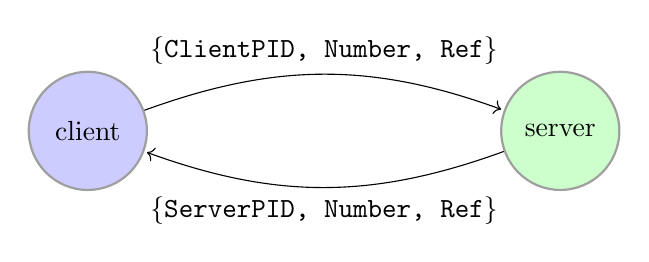
\begin{tikzpicture}[shorten >=1pt,node distance=6cm,on grid,
    every state/.style={draw=blue!50,very thick,fill=blue!20}]
  \tikzstyle{nodeI}=[circle,thick,draw=gray!75,fill=blue!20,minimum size=15mm]
  \tikzstyle{nodeC}=[circle,thick,draw=gray!75,fill=green!20,minimum size=15mm]
 
  \node[nodeI]          (client)              {client};
  \node[nodeC]          (server) [right=of client] {server}; 
 
  \path[->] (client) edge [bend left=20] node [above] {\texttt{\{ClientPID, Number, Ref\}}} (server);
  \path[->] (server) edge [bend left=20] node [below] {\texttt{\{ServerPID, Number, Ref\}}} (client);
\end{tikzpicture}
}
\caption{Multiplying number in request by 2}
%\vspace{-15pt}
\label{fig:by2server}
\end{figure}

As we can see, this program is following the \texttt{Erlang} conventions of
attaching references to the messages, so we can easily detect which messages
are causally related. Therefore, we can clearly see which messages belong to
the same chain of messages. This association is precisely what we mean by
different chains of messages. Even if the same client interacts again with the
system, the chain will still be considered an isolated chain from the others.

Consider $\sigma_1$ and $\sigma_2$, where the latter was produced by a
faulty implementation of the \texttt{server} process.
\[
\begin{align*}
\sigma_1 = \textcolor{black}{\texttt{\{client1, 10, \#1\}}} \
\textcolor{black}{\texttt{\{client2, 20, \#2\}}} \
\textcolor{black}{\texttt{\{server, 40, \#2\}}} \
\textcolor{black}{\texttt{\{server, 20, \#1\}}} \\
\sigma_2 = \textcolor{black}{\texttt{\{client1, 10, \#1\}}} \
\textcolor{black}{\texttt{\{client2, 20, \#2\}}} \
  \textcolor{black}{\texttt{\{server, \textcolor{red}{20}, \#2\}}} \
\textcolor{black}{\texttt{\{server, 20, \#1\}}} 
\end{align*}
\]

Depending on whether the system is correctly implemented, it will adhere to the
property that we expect, which is returning the original number multiplied by
two. This can be specified by the following property:
\[
\varphi =
\Omega\left(
\begin{aligned}
 &\text{\texttt{send$_{\text{client} \rightarrow \text{server}}$}}\{\_, \text{\texttt{Number, Ref}}\} : \top\ ; \\
 &\quad\text{\texttt{send$_{\text{server} \rightarrow \text{client}}$}}\{\_, \text{\texttt{NumberReturn, Ref}}\} :
   \text{\texttt{NumberReturn = 2 * Number}}
\end{aligned}
\right)
\]

Since every message chain operates within the same context, the $\Omega$ modal
operator evaluates whether all contexts, that is, all individual message
chains, satisfy a given property. By specifying the property $\varphi$, we can
capture the desired system behaviour. In the runtime setting, the monitor
generated from $\varphi$ continuously checks for violations. If no violation
occurs in the observed trace, the monitor outputs the inconclusive verdict
"\texttt{?}".

Under this framework, the property $\varphi$ is not violated in trace
$\sigma_1$, whereas it is violated in trace $\sigma_2$ because one of the
message chains fails to satisfy the boolean constraint defined by $\varphi$.
This example illustrates how message chains are tracked and interpreted by the
WALTZ monitor, highlighting the role of causal context in runtime
verification.
\subsection{Filtering Chains - Turning Infinity Into Finity}
\label{sub_sec:filteringchains}
Before moving on, it is of great importance to understand how messages will
exist within the different contexts. The trace is a potentially infinite entity
that grows continuously as the system executes. However, for evaluations within
different contexts, the message chain inside each context is treated as a
finite trace.

We will be working with sub-traces, which compose the main trace being produced
by the system. The internal mechanisms will automatically filter all the
relevant messages present in the specification of a property to compose this
sub-trace. We can think of this as messages flowing into the right place, that
is, into the right context. Of course, message chains can be extremely long,
but realistically they have a reasonable finite size.

This does not mean that the overall trace will be treated as finite. Rather,
the intention is that the root context, $\Delta_0$, may have infinitely many
child contexts, but within each child context, the corresponding message chain
is regarded as finite. Consider the trace $\sigma = \_ \
\textcolor{black}{\texttt{m$_1$}} \ \_ \ \_ \ \textcolor{black}{\texttt{m$_2$}}
\ \_ \ \_ \ \textcolor{black}{\texttt{m$_3$}} \ \_ \ \_ \
\textcolor{black}{\texttt{m$_4$}}$ with the following context assignments
$\gamma(\text{\texttt{m$_1$}}) = \Delta_1, \gamma(\text{\texttt{m$_2$}}) =
\Delta_2, \gamma(\text{\texttt{m$_3$}}) = \Delta_1,
\gamma(\text{\texttt{m$_4$}}) = \Delta_2$.

In this case, the messages belonging to the same context preserve their
relative order. For example, within $\Delta_1$, message $\texttt{m$_1$}$
precedes $\texttt{m$_3$}$, while in $\Delta_2$, $\texttt{m$_2$}$ precedes
$\texttt{m$_4$}$. Thus, although the global trace may be infinite, each context
isolates a finite, ordered chain of messages that can be reasoned about
independently. The structuring of our context tree $\mathcal{C}$, is visible in
\Cref{fig:contextmanagement}, which highlights the idea of the
$\blacktriangleright$ association between the contexts in the system, in this
case, $\Delta_1 \blacktriangleright \Delta_0$ and $\Delta_2 \blacktriangleright
\Delta_0$.

\begin{figure}[ht]
\centering
\usetikzlibrary{arrows.meta, positioning, automata, shapes.geometric}
\scalebox{1}{%
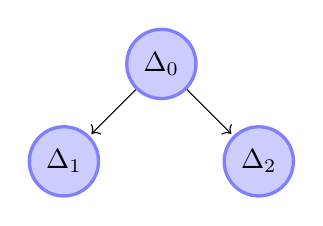
\begin{tikzpicture}[shorten >=1pt,node distance=1.75cm,on grid,
    every state/.style={draw=blue!50,very thick,fill=blue!20}]
  \tikzstyle{nodeG}=[circle,thick,draw=gray!75,fill=green!20,minimum size=10mm]
  \tikzstyle{nodeR}=[circle,thick,draw=gray!75,fill=red!20,minimum size=10mm]
  \tikzstyle{nodeB}=[circle,thick,draw=gray!75,fill=blue!20,minimum size=10mm]
  \tikzstyle{nodeI}=[state, circle,thick,draw=gray!75,fill=blue!20,minimum size=10mm]
 
  \node[nodeI, state]          (q_000)              {$\Delta_0$};
  \node[nodeB, state]          (q_111) [below right=of q_000] {$\Delta_2$};
  \node[nodeB, state]          (q_222) [below left=of q_000] {$\Delta_1$}; 

  \path[->] (q_000) edge node [above right]  {} (q_111);
  \path[->] (q_000) edge node [above left] {} (q_222);
 
\end{tikzpicture}
}
  \caption{Context tree of the trace $\sigma$ given by $\mathcal{C}$ }
%\vspace{-10pt}
\label{fig:contextmanagement}
\end{figure}

In order to have a clear understanding of how these contexts exist and are
"bound" to message chains, consult \Cref{fig:contextmanagement_evolution} which
depicts a step by step context tree creation that eases the understanding of
this concept. Each message is routed to its appropriate context, and if no such
context exists, a new one is created to host the corresponding message chain.

\begin{figure}[ht]
\centering
\usetikzlibrary{arrows.meta, positioning, automata, shapes.geometric}

% Define styles
\tikzstyle{nodeG}=[circle,thick,draw=gray!75,fill=green!20,minimum size=10mm]
\tikzstyle{nodeR}=[circle,thick,draw=gray!75,fill=red!20,minimum size=10mm]
\tikzstyle{nodeB}=[circle,thick,draw=gray!75,fill=blue!20,minimum size=10mm]
\tikzstyle{nodeI}=[state, circle,thick,draw=gray!75,fill=blue!20,minimum size=10mm]

% Step 1: Only Delta_0
\begin{subfigure}[b]{0.3\textwidth}
\centering
\scalebox{1}{%
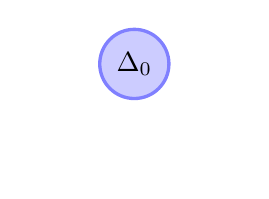
\begin{tikzpicture}[shorten >=1pt,node distance=1.75cm,on grid,
    every state/.style={draw=blue!50,very thick,fill=blue!20}]
  \node[nodeI, state] (q_000) {$\Delta_0$};
  % Invisible nodes to maintain consistent positioning
  \node[opacity=0] (q_111) [below right=of q_000] {};
  \node[opacity=0] (q_222) [below left=of q_000] {}; 
\end{tikzpicture}
}
\caption{Initial state}
\end{subfigure}
%
% Step 2: Delta_1 appears with m1
\begin{subfigure}[b]{0.3\textwidth}
\centering
\scalebox{1}{%
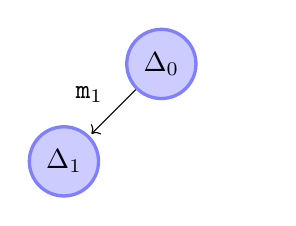
\begin{tikzpicture}[shorten >=1pt,node distance=1.75cm,on grid,
    every state/.style={draw=blue!50,very thick,fill=blue!20}]
  \node[nodeI, state] (q_000) {$\Delta_0$};
  \node[nodeB, state] (q_222) [below left=of q_000] {$\Delta_1$}; 
  % Invisible node to maintain consistent positioning
  \node[opacity=0] (q_111) [below right=of q_000] {};
  \path[->] (q_000) edge node [above left] {\texttt{m$_1$}} (q_222);
\end{tikzpicture}
}
\caption{$\Delta_1$ creation}
\end{subfigure}
%
% Step 3: Delta_2 appears with m2
\begin{subfigure}[b]{0.3\textwidth}
\centering
\scalebox{1}{%
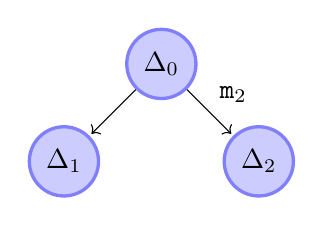
\begin{tikzpicture}[shorten >=1pt,node distance=1.75cm,on grid,
    every state/.style={draw=blue!50,very thick,fill=blue!20}]
  \node[nodeI, state] (q_000) {$\Delta_0$};
  \node[nodeB, state] (q_111) [below right=of q_000] {$\Delta_2$};
  \node[nodeB, state] (q_222) [below left=of q_000] {$\Delta_1$}; 
  \path[->] (q_000) edge node [above right] {\texttt{m$_2$}} (q_111);
  \path[->] (q_000) edge node [above left] {} (q_222);
\end{tikzpicture}
}
\caption{$\Delta_2$ creation}
\end{subfigure}

\vspace{1cm}

% Step 4: Transition to Delta_1 changes to m3
\begin{subfigure}[b]{0.3\textwidth}
\centering
\scalebox{1}{%
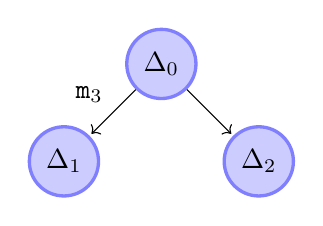
\begin{tikzpicture}[shorten >=1pt,node distance=1.75cm,on grid,
    every state/.style={draw=blue!50,very thick,fill=blue!20}]
  \node[nodeI, state] (q_000) {$\Delta_0$};
  \node[nodeB, state] (q_111) [below right=of q_000] {$\Delta_2$};
  \node[nodeB, state] (q_222) [below left=of q_000] {$\Delta_1$}; 
  \path[->] (q_000) edge node [above right] {} (q_111);
  \path[->] (q_000) edge node [above left] {\texttt{m$_3$}} (q_222);
\end{tikzpicture}
}
\caption{$\Delta_1$ routing}
\end{subfigure}
%
% Step 5: Transition to Delta_2 changes to m4
\begin{subfigure}[b]{0.3\textwidth}
\centering
\scalebox{1}{%
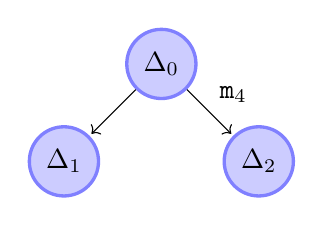
\begin{tikzpicture}[shorten >=1pt,node distance=1.75cm,on grid,
    every state/.style={draw=blue!50,very thick,fill=blue!20}]
  \node[nodeI, state] (q_000) {$\Delta_0$};
  \node[nodeB, state] (q_111) [below right=of q_000] {$\Delta_2$};
  \node[nodeB, state] (q_222) [below left=of q_000] {$\Delta_1$}; 
  \path[->] (q_000) edge node [above right] {\texttt{m$_4$}} (q_111);
  \path[->] (q_000) edge node [above left] {} (q_222);
\end{tikzpicture}
}
\caption{$\Delta_2$ routing}
\end{subfigure}
%
% Empty space for 2x3 grid alignment
\begin{subfigure}[b]{0.3\textwidth}
\centering
% Empty subfigure for grid alignment
\end{subfigure}
\caption{Evolution of the context tree showing the dynamic construction process}
\label{fig:contextmanagement_evolution}
\end{figure}

Each sub-trace within a context has a well-defined beginning, marked by the
anchor of its message chain, and a corresponding end, which enables the
verification of properties over these finite segments. As we will see later,
this property holds particularly for the leaf nodes of the context tree. Once
hierarchical relations are introduced, however, new sub-traces may no longer
have a natural endpoint and can instead grow indefinitely. This aspect will be
examined in more detail in \Cref{sec:waltz_nesting}.

This constitutes our mechanism of verification: traversing the different
contexts and checking properties over them. Depending on the chosen operator,
verification may require ensuring compliance across all contexts or identifying
at least one context where the property holds. These ideas anticipate the modal
operators of WALTZ, which are discussed in detail in \Cref{sec:waltz_modalop}.

\subsection{Why Context Matters?}
\label{sub_sec:waltz_context}

The concept of a context is central to verifying the satisfiability of a WALTZ
formula. As previously discussed, the main context, denoted $\Delta_0$, always
exists and can be regarded as representing the system. It acts as a primary
reference point, or oracle, for verification. Whenever a new context is
introduced, hierarchical relationships are automatically established between it
and existing contexts. The evaluation of properties then depends on the chosen
operator, such as $\Omega$ or $\Theta$. Therefore, in order to evaluate a WALTZ
formula, the entities that exist are the trace $\sigma$, the context tree
$\mathcal{C}$, and the mapping from the messages to the respective context
function $\gamma$. For now, this is simply a mathematical function that maps
messages to the respective context.

Understanding the context verification mechanism and how it aids and supports
the property satisfiability is of great importance since it is the core of our
language and verification process in concurrent systems. In this section,
whenever we associate a colour to a message it means that it belong to a given
context, therefore, all messages sharing the same colour belong to the same
context. We also use a simple notation to denote the satisfaction or violation
of boolean constraints, using the symbol \ding{52} for satisfaction and
\ding{56} for violation, and irrelevant messages produced by the system are symbolised by \texttt{\_}.

\begin{example}
The system architecture is designed around a central server that routes
  incoming requests to specialized worker processes. In this simplified
  implementation, the server receives an input list and delegates it to a
  worker that removes duplicate values. The resulting duplicate-free list is
  then passed to another worker responsible for sorting. Together, these
  components ensure that the final output is both free of duplicates and
  properly ordered. The overall workflow is illustrated in
  \Cref{fig:introexamplelists}.
\end{example}
%
\begin{figure}[htbp]
\centering
\usetikzlibrary{arrows.meta,automata,positioning}
\scalebox{0.85}{%
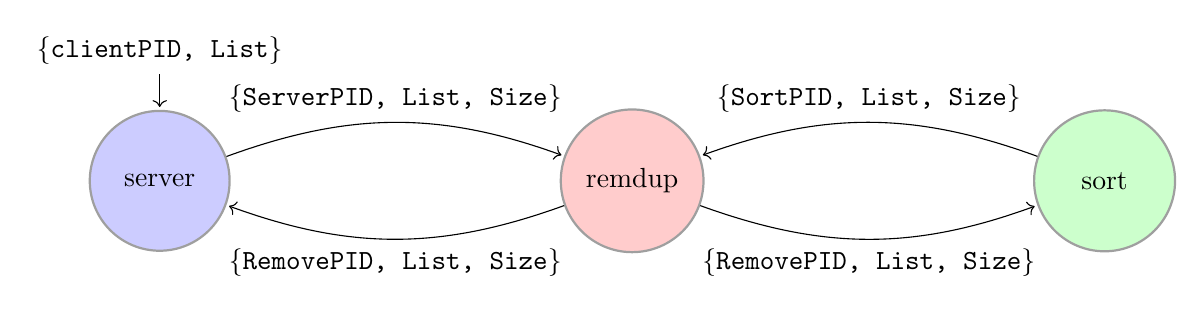
\begin{tikzpicture}[shorten >=1pt,node distance=6cm,on grid,
    every state/.style={draw=blue!50,very thick,fill=blue!20}]
  \tikzstyle{nodeB}=[circle,thick,draw=gray!75,fill=red!20,minimum size=15mm, text width=15mm, align=center]
  \tikzstyle{nodeI}=[circle,thick,draw=gray!75,fill=blue!20,minimum size=15mm, text width=15mm, align=center]
  \tikzstyle{nodeC}=[circle,thick,draw=gray!75,fill=green!20,minimum size=15mm, text width=15mm, align=center]
 
  \node[nodeI]          (server)              {server};
  \node[nodeB]          (remdup) [right=of server] {remdup};
  \node[nodeC]          (sort) [right=of remdup] {sort}; 

  \path[->] 
      (server.north) ++(0,0.75) node (start) {\texttt{\{clientPID, List\}}} 
      edge (server.north);
      
  \path[->] (server) edge [bend left=20] node [above] {\texttt{\{ServerPID, List, Size\}}} (remdup);
  \path[->] (remdup) edge [bend left=20] node [below] {\texttt{\{RemovePID, List, Size\}}} (server);
  \path[->] (remdup) edge [bend right=20] node [below] {\texttt{\{RemovePID, List, Size\}}} (sort);
  \path[->] (sort) edge [bend right=20] node [above] {\texttt{\{SortPID, List, Size\}}} (remdup);
  %\path[->] (sort) edge [bend left=20] node [below] {\texttt{\{sortPID, List, Size\}}} (remove);
\end{tikzpicture}
}
\caption{Actor-based system that operates over a list}
%\vspace{-15pt}
\label{fig:introexamplelists}
\end{figure}

We will use the dummy system from \Cref{fig:introexamplelists} throughout this
section to ease the explanation of context aware verification and the necessity
of having it. At first, let us ignore completely the context management, that is, the
function $\gamma$ will assign the same global context to all the messages of our interest that
come from the system trace. Consider the trace $\sigma_1$ depicted below: 
$$
\sigma_1 = \_ \ \textcolor{black}{\texttt{m$_1$}} \ \_ \ \_ \ \textcolor{black}{\texttt{m$_2$}} \ \_ \ \_ \ \textcolor{black}{\texttt{m$_3$}} \ ... 
$$

If we wanted to evaluate property $\varphi_1 = \Omega(\alpha : \delta)$, over
trace $\sigma_1$, the evaluation of this property actually depends on how the
context is assigned to each message. What we would like to capture with this
property is that "for every context, we want to check that if there exists a
message with signature $\alpha$ it adheres to the boolean constraint $\delta$".
In the case of our system, a property of such kind could be "all the lists
exiting the \texttt{sort} process are sorted". Now here is the nuance, if the
context mapping for the messages is $\gamma( \text{\texttt{m$_1$}}) =
\Delta_{1}$, $\gamma( \text{\texttt{m$_2$}}) = \Delta_{1}$, and $\gamma(
\text{\texttt{m$_3$}}) = \Delta_{1}$, that is, they all share the same context,
and assume that all the messages have signature $\alpha$, which is the one we
are trying to capture. What would result of the verification of trace
$\sigma_1$ with the boolean constraints present in the trace $\sigma_1$ is the
satisfaction of the property $\varphi_1$.
\[
\sigma_1 = \_ \ \textcolor{blue}{\texttt{m$_1$}}^{\text{\ding{56}}} \ \_ \ \_
         \ \textcolor{blue}{\texttt{m$_2$}}^{\text{\ding{56}}} \ \_ \ \_
         \ \textcolor{blue}{\texttt{m$_3$}}^{\text{\ding{52}}} ...
\]

The property $\varphi_1$ is satisfied under the conditions present, due to the following semantic rule: 
$$
\sigma, \Delta \;&\models\; \alpha : \delta \text{ iff } \exists_{i \geq 0} : \sigma_i \models \delta \text{ and } \sigma_i \bowtie \alpha \text{ and } \gamma(\sigma_i) = \Delta
$$

In this case, we only need to identify a message within the context that
fulfills the property. This is exactly what occurs in the trace, since
\texttt{m$_3$} satisfies $\delta$, thereby ensuring the property holds for the
entire context. Drawing a parallel with our earlier example, under the current
interpretation, where all messages are assigned to the same context, we risk
allowing unsorted lists. This is because the property would be considered
satisfied as long as at least one list is sorted, even if others are not.

However, that is not what we actually want to represent with property
$\varphi_1$; we would like to have the verification that \textbf{every} message
that has signature $\alpha$, satisfies $\delta$, essentially isolating every
message with signature $\alpha$ in its own separate context from the others. To
achieve this, we introduce the notion of context by redefining the context
mapping as follows: $\gamma(\texttt{m$1$}) = \Delta{1}$, $\gamma(\texttt{m$2$})
= \Delta{2}$, and $\gamma(\texttt{m$3$}) = \Delta{3}$. With these mappings in
place, we are now verifying the intended requirement: that for every message
with signature $\alpha$, the property must hold. In the case of the trace
$\sigma_1$, this ensures the property is immediately violated, since two of the
messages fail to satisfy $\delta$.
\[
\sigma_1 = \_ \ \textcolor{blue}{\texttt{m$_1$}}^{\text{\ding{56}}} \ \_ \ \_
         \ \textcolor{red}{\texttt{m$_2$}}^{\text{\ding{56}}} \ \_ \ \_
         \ \textcolor{orange}{\texttt{m$_3$}}^{\text{\ding{52}}} ...
\]

One might ask: what is the correct way to assign contexts? In fact, there is no
single correct way, as context assignment occurs at runtime and establishes the
causal relations between messages. The monitors, generated from the specified
properties, then interpret these contexts according to how the property is
defined. More precisely, they interpret the \textbf{chains} of messages that
are causally related, as determined by the function $\gamma$. For now, we will
treat this as given, but in \Cref{cha:actorchestra} we will explore in detail
how the $\gamma$ operates.

Our context management strategy assigns the same context to all messages
belonging to the same chain. Consequently, when we have $\alpha : \delta$, each
message with signature $\alpha$ resides in its own context, since in this case
the “chain” consists solely of the message itself. Recall that whenever we
specify $\varphi_2 = \alpha_{1} : \delta_{1} \ ; \ \alpha_{2} : \delta_{2}$,
the chain becomes unbreakable. This means that if, at any point within the
chain, a boolean constraint is not satisfied, the chain is considered broken,
and verification must continue with another chain from a different context.
Depending on the monitored property, such a break may constitute a violation.
For instance, if we are monitoring $\Omega(\varphi_2)$, then the violation of a
single chain would cause the entire property to be violated.

We can think of this in the same way as \texttt{Erlang} interactions, where
each request lives in its own bubble, these bubbles correspond to our contexts.
For every chain (interaction), we assign a dedicated bubble in which
verification takes place.

To have another perspective on this and understand how it works for the
$\Theta$ operator consider property $\varphi_2 = \Theta(\alpha_{1} : \delta_{1}
\ ; \ \varphi_{2} : \delta_{2})$, over the following trace: $$ \sigma_2 = \_ \
\textcolor{blue}{\texttt{m$_1$}} \ \_ \ \_ \ \textcolor{red}{\texttt{m$_2$}}
\ \_ \ \_ \ \textcolor{blue}{\texttt{m$_3$}} \ \_ \ \_ \
\textcolor{red}{\texttt{m$_4$}} \ ... $$

and the context mapping: $\gamma(\text{\texttt{m$_1$}}) = \Delta_1,
\gamma(\text{\texttt{m$_2$}}) = \Delta_2, \gamma(\text{\texttt{m$_3$}}) =
\Delta_1, \gamma(\text{\texttt{m$_4$}}) = \Delta_2$, which is depicted by
$\mathcal{C}$ in \Cref{fig:contextmanag}.

\begin{figure}[ht]
\centering
\usetikzlibrary{arrows.meta, positioning, automata, shapes.geometric}
\scalebox{1}{%
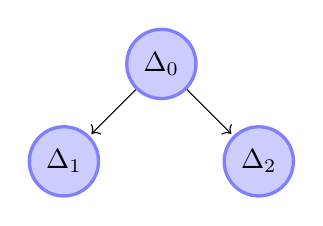
\begin{tikzpicture}[shorten >=1pt,node distance=1.75cm,on grid,
    every state/.style={draw=blue!50,very thick,fill=blue!20}]
  \tikzstyle{nodeG}=[circle,thick,draw=gray!75,fill=green!20,minimum size=10mm]
  \tikzstyle{nodeR}=[circle,thick,draw=gray!75,fill=red!20,minimum size=10mm]
  \tikzstyle{nodeB}=[circle,thick,draw=gray!75,fill=blue!20,minimum size=10mm]
  \tikzstyle{nodeI}=[state, circle,thick,draw=gray!75,fill=blue!20,minimum size=10mm]
 
  \node[nodeI, state]          (q_000)              {$\Delta_0$};
  \node[nodeB, state]          (q_111) [below right=of q_000] {$\Delta_2$};
  \node[nodeB, state]          (q_222) [below left=of q_000] {$\Delta_1$}; 

  \path[->] (q_000) edge node [above right]  {} (q_111);
  \path[->] (q_000) edge node [above left] {} (q_222);
 
\end{tikzpicture}
}
  \caption{Context tree of the trace $\sigma_2$ given by $\mathcal{C}$ }
%\vspace{-10pt}
\label{fig:contextmanag}
\end{figure}

Each context will have a dedicated monitor that checks the property
\(\alpha_{1} : \delta_{1}\) and \(\alpha_{2} : \delta_{2}\) individually,
recreating the chain. In the next chapter, we will explore how this process is
carried out. Each monitor will receive only the filtered messages that are
necessary for its contextual interpretation, resulting in finite sub-traces for
evaluation, as illustrated in \Cref{fig:waltz_monitorstruct}. Within each
context, we will assess the specified property; while the overall trace
continuously grows, the interpretation for each message chain remains finite.
Although the number of chains produced is infinite, we are grouping them and
directing them to the appropriate monitor to verify property satisfaction.
Thus, even if the root context has an infinite number of children, each child
context will have a finite perspective on the global trace of the system.

\begin{figure}[ht]
\centering
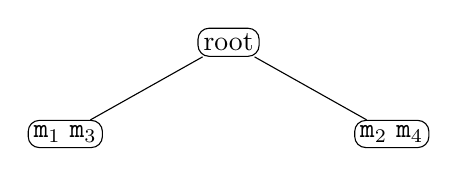
\begin{tikzpicture}[node distance=0.8cm and 1.2cm, every node/.style={draw, rounded corners, inner sep=2pt}]
    % Top node
    \node (oracle) {root};
    % Bottom-left node
    \node (leftab) [below left=of oracle] {\texttt{m$_1$} \texttt{m$_3$}};
    % Bottom-right node
    \node (rightab) [below right=of oracle] {\texttt{m$_2$} \texttt{m$_4$}};

    % Edges
    \draw (oracle) -- (leftab);
    \draw (oracle) -- (rightab);
\end{tikzpicture}
\caption{The monitor structure for property $\varphi_2$}
\label{fig:waltz_monitorstruct}
\end{figure}

Assume that \texttt{m$_1$}, \texttt{m$2$} $\bowtie \alpha{1}$ and
\texttt{m$_3$}, \texttt{m$4$} $\bowtie \alpha{2}$, with the boolean constraints
evaluated as follows:
\[
\sigma_2 = \_ \ \textcolor{blue}{\texttt{m$_1$}}^{\text{\ding{52}}} \ \_ \ \_
         \ \textcolor{red}{\texttt{m$_2$}}^{\text{\ding{52}}} \ \_ \ \_
         \ \textcolor{blue}{\texttt{m$_3$}}^{\text{\ding{56}}} \ \_ \ \_
         \ \textcolor{red}{\texttt{m$_4$}}^{\text{\ding{52}}} ...
\]

In this scenario, the property is satisfied because at least one context,
namely $\Delta_2$, adheres to it. However, if all these messages are placed in
the same context, that is, no context management exists whatsoever, the
situation changes. Consider the same trace, but with new boolean outcomes:
\[
\sigma_2 = \_ \ \textcolor{blue}{\texttt{m$_1$}}^{\text{\ding{52}}} \ \_ \ \_
         \ \textcolor{blue}{\texttt{m$_2$}}^{\text{\ding{56}}} \ \_ \ \_
         \ \textcolor{blue}{\texttt{m$_3$}}^{\text{\ding{56}}} \ \_ \ \_
         \ \textcolor{blue}{\texttt{m$_4$}}^{\text{\ding{52}}} ...
\]

At first glance, this trace would be accepted as satisfying the property. Yet
this interpretation is misleading. If \texttt{m$_1$} and \texttt{m$_3$} are
causally related (thus belong to the same context), and likewise \texttt{m$_2$}
and \texttt{m$_4$}, then within each causal chain the property is never
satisfied. In other words, under proper context management, the monitor should state
inconclusiveness. Treating all messages as part of a single context therefore produces
incorrect verdicts that do not reflect the true causal structure.

To draw a parallel with our example, consider the trace of interactions from
two different clients with the system. These interactions can be represented by
the sub-traces $\sigma_{\text{\texttt{c1}}}$ and $\sigma_{\text{\texttt{c2}}}$.
In this case, the traces reflect a buggy version of the system, where the lists
of data between the two clients are inadvertently swapped.
\[
\begin{align*}
\sigma_{\text{\texttt{c1}}} = \textcolor{black}{\texttt{\{<0.1.0>, [1,2,2], 3\}}} \ \textcolor{black}{\texttt{\{<0.2.0>, [5,1,3], 3\}}} \\
  \sigma_{\text{\texttt{c2}}} = \textcolor{black}{\texttt{\{<0.1.0>, [5,1,3,5], 4\}}} \ \textcolor{black}{\texttt{\{<0.2.0>, [1,2], 2\}}} 
\end{align*}
\]
\iffalse
\textcolor{black}{\texttt{\{<0.1.0>, [1,2,2], 3\}}}^{\text{\ding{52}}} \\ 
\textcolor{black}{\texttt{\{<0.1.0>, [5,1,3,5], 4\}}}^{\text{\ding{52}}} \\
\textcolor{black}{\texttt{\{<0.2.0>, [1,2], 2\}}}^{\text{\ding{52}}} \\
\textcolor{black}{\texttt{\{<0.2.0>, [5,1,3,5], 4\}}}^{\text{\ding{56}}}
\fi

One property of interest is whether the \texttt{remdup} process correctly
removes all duplicates from the original list, denoted by $\varphi$. This can
be verified by comparing the list received by \texttt{remdup} from the
\texttt{server} with the list it subsequently sends to \texttt{sort}, ensuring
that all duplicates have been eliminated.

Considering that there is no context management, that is, all the messages
belong to the same context, observing both sub-traces, we can see that the
lists get swapped for both the clients, due to a buggy management of the
\texttt{remdup} process. If we were to verify $\Theta(\varphi)$, the property
would be satisfied, since all the messages are evaluated within the same
context. But, that is definitely not the case, since individually, none of the
client interactions respected the property $\varphi$.

The issue of not having context management is that we become prone to erroneous
verdicts, as illustrated above. This underscores the necessity of relating each
causal chain individually, so that information from one context is not mixed
with another, avoiding false verdicts by the monitor. This is precisely why
context plays a critical role in the verification process. We explore how
context is managed in \Cref{cha:actorchestra}.

\iffalse
We have to think about this, as the notion of unreakability of each chain.
Whenever a chain is established, it will have a beginning and an ending, the
chains will be like atomic chunks of multiple messages that are all interpreted
within the same context. For example, having $\Omega(\alpha : \delta)$, means
that we will interpret the trace as single individual messages, with signature
$\alpha$, and each one of them is going to be interpreted within a different
context. We will not allow room, for an $\alpha$ observation, to "live" more
than it should. 
\fi

\iffalse
If, for instance, we wanted to verify property $\varphi_3 = \Omega(\alpha_{1} :
\delta_{1} \ ; \ \varphi_{2} : \delta_{2})$ over the same trace and context 
mapping, for the following boolean constraint satisfactions:

\[
\sigma = \_ \ \textcolor{blue}{\texttt{m$_1$}}^{\text{\ding{52}}} \ \_ \ \_
         \ \textcolor{red}{\texttt{m$_2$}}^{\text{\ding{52}}} \ \_ \ \_
         \ \textcolor{blue}{\texttt{m$_3$}}^{\text{\ding{56}}} \ \_ \ \_
         \ \textcolor{red}{\texttt{m$_4$}}^{\text{\ding{52}}} ...
\]

the property $\varphi_3$ would not be satisfied, because one of the contexts does not
satisfy the property $\alpha_{1} : \delta_{1} \ ; \ \alpha_{2} : \delta_{2}$.
\fi
\iffalse
The context management will be there no matter what, it is something that has 
to exist alongside the trace being provided. The way that we verify and interpret 
the trace of events based on these contexts is what changes from property to
property.
\fi

\iffalse
Consider $\varphi_1 = \alpha : \delta$ and the following trace (where \_ is an
irrelevant message): 
$$
\sigma_1 = \_ \ \textcolor{red}{\texttt{m$_1$}} \ \_ \ \_ \ \textcolor{red}{\texttt{m$_2$}}
$$
In $\sigma_1$, all the messages with signature $\alpha$ belong to the same context ($\Delta_0$). To satisfy $\varphi_1$, it is sufficient to check whether in the trace, there is at least one of them that satisfies the property $\delta$. Some messages may not satisfy $\delta$, but as long as at least one does, the formula is considered satisfied.

Now, consider the same trace, but suppose the goal is to check all messages with signature $\alpha$ that adhere to $\delta$. In this case, the property would be defined as $\varphi_2 = \Omega (\alpha : \delta)$, and the contexts would change, as such:
$$
\sigma_2 = \_ \ \textcolor{red}{\texttt{m$_1$}}  \ \_ \ \_ \ \textcolor{blue}{\texttt{m$_2$}} 
$$
The objective is to verify property $\delta$ over all messages with signature
$\alpha$. In this example, there are two existing contexts, the context of
the message \textcolor{red}{\texttt{m$_1$}} matching \textcolor{red}{$\alpha$}, denoted by $\Delta_1$, and the context of
the message \textcolor{blue}{\texttt{m$_2$}}  matching \textcolor{blue}{$\alpha$}, denoted by $\Delta_2$. These contexts, each
represented by a different colour, are independent, which is precisely what is
needed. Each occurrence of the message chain defined within the $\Omega$
operator is evaluated as a separate context, ensuring that the property is
checked individually for every instance.

In $\varphi_1$, even if the first message matching the signature does not
satisfy the property, the formula is still satisfied as long as at least one
subsequent message does. This is not the case for $\varphi_2$, where it is
required that the property holds for every independent chain. Now, let us consider trace
$\sigma_3$ as:
$$
\sigma_3 = \textcolor{red}{\texttt{m$_1$}}  \ \_ \ \textcolor{red}{\texttt{m$_2$}}  \ \_ \ \textcolor{blue}{\texttt{m$_3$}}  \ 
\_ \ \_ \ \textcolor{red}{\texttt{m$_4$}}  \ \_ \ \textcolor{blue}{\texttt{m$_5$}} 
$$
We can interpret $\sigma_3$ with respect to property $P$: \textit{``For
every client connected to the system, all requests sent by that client must
have a positive payload''}. In WALTZ, this is expressed as: $\varphi_3 =
\Omega(\alpha_1 : \top ; \Omega(\alpha_2 : \delta))$.

Property $\varphi_3$ uses two nested $\Omega$ operators, essential for
correctly capturing the intended behaviour. The outer $\Omega$ tracks each
client connection $\alpha_1$, matching messages \textcolor{red}{\texttt{m$_1$}}
and \textcolor{blue}{\texttt{m$_3$}}. The inner $\Omega$ tracks the sequence of
requests $\alpha_2$, matching the remaining messages. Without the second
$\Omega$, the formula would monitor all requests globally rather than per
client, thus failing to isolate behaviours across individual connections.
The resulting structure of contexts derived from this trace and property is
illustrated in \Cref{fig:latticecontext2}, which shows the hierarchical
relationships established by the nested $\Omega$ operators.

\begin{figure}[t]
\centering
\usetikzlibrary {arrows.meta,automata,positioning}
\scalebox{0.8}{%
\begin{tikzpicture}[shorten >=1pt,node distance=1.25cm,on grid,
    every state/.style={draw=blue!50,very thick,fill=blue!20}]
  \tikzstyle{nodeG}=[circle,thick,draw=gray!75,fill=green!20,minimum size=10mm]
  \tikzstyle{nodeR}=[circle,thick,draw=gray!75,fill=red!20,minimum size=10mm]
  \tikzstyle{nodeB}=[circle,thick,draw=gray!75,fill=blue!20,minimum size=10mm]
  \tikzstyle{nodeI}=[state, circle,thick,draw=gray!75,fill=blue!20,minimum size=10mm]
 
  \node[nodeI, state]          (q_000)              {$\Delta_0$};
  \node[nodeB, state]          (q_111) [below right=of q_000] {$\Delta_2$};
  \node[nodeB, state]          (q_222) [below left=of q_000] {$\Delta_1$}; 
  \node[nodeG, state]          (q_333) [below left= of q_222] {$\Delta_{11}$}
  \node[nodeG, state]          (q_555) [below right= of q_222] {$\Delta_{12}$}
  \node[nodeG, state]          (q_666) [below right = of q_111] {$\Delta_{21}$}
 

  \path[->] (q_000) edge node [above right]  {} (q_111);
  \path[->] (q_000) edge node [above left] {} (q_222);
  \path[->] (q_222) edge node [above right] {} (q_555);
  \path[->] (q_222) edge node [above left] {} (q_333);
  \path[->] (q_111) edge node [above right] {} (q_666);

\end{tikzpicture}
}
\caption{The contexts of the trace $\sigma_3$}
%\vspace{-10pt}
\label{fig:latticecontext2}
\end{figure}

The context $\Delta_0$ is the root context and is always present in any trace.
For example, a simple formula like $\varphi = \alpha_1 : \delta$ is evaluated
within this root context $\Delta_0$. However, when a formula involves the
$\Omega$ operator, it introduces a new context that inherits the context in
which it was invoked. Each client initiates a chain of events matched by the
formula $\alpha : \top ; \Omega(\alpha_2 : \delta)$. Upon observing an event
that satisfies $\alpha : \top$, a new context is created, denoted $\Delta_1$,
with $\Delta_0$ as its parent, i.e., $\Delta_1 \blacktriangleright \Delta_0$.
This context captures the interaction scope for a single client.

The formula then specifies another use of $\Omega$, which applies to all
subsequent messages from that client. For each message matching $\alpha_2$, we
create a new sub-context (e.g., $\Delta_{11}$, $\Delta_{12}$) under $\Delta_1$,
since we are now verifying whether each of those messages satisfies the
property $\delta$. These new contexts inherit from $\Delta_1$, meaning
$\Delta_{11} \blacktriangleright \Delta_1$ and $\Delta_{12} \blacktriangleright
\Delta_1$. This hierarchical context structure enables us to handle traces
where events from different chains or clients are interleaved, as
satisfiability is always checked within the relevant context. Therefore, in
$\sigma_{3}$, one of the interaction is \textcolor{red}{\texttt{m$_1$}} ;
\textcolor{red}{\texttt{m$_2$}} ; \textcolor{red}{\texttt{m$_4$}} and the other
one is \textcolor{blue}{\texttt{m$_3$}} ; \textcolor{blue}{\texttt{m$_5$}}.

\iffalse
For example, to verify the property for the first client: we check that $\alpha : \top$ holds in context $\Delta_1$, and then that each $\alpha'$ message satisfies $\delta$ in its respective sub-contexts, $\Delta_{11}$ and $\Delta_{12}$. Since both sub-contexts are children of $\Delta_1$, and $\Delta_1$ is itself derived from $\Delta_0$, the full property is validated along the intended hierarchy of contexts.
\fi
\fi

\section{The Modal Operators $\Omega$ and $\Theta$}
\label{sec:waltz_modalop}
Now that we have established the notions of message chains and the role of
contexts, we can turn to the modal operators of WALTZ and examine how they
enable the verification of different classes of properties. As discussed,
multiple contexts may coexist throughout the lifespan of the system, and our
verification process operates over these contexts.

In some cases, we may wish to express that all message chains must satisfy a
given property; in others, it may be sufficient that at least one message chain
does so. The modal operators provide exactly this expressive power, allowing us
to capture such requirements in a precise and systematic way.
\subsection{The $\Theta$ Operator}
\label{sub_sec:waltz_thetaop}
Whenever we use $\Theta(\varphi)$, we are stating that we want to see the
satisfaction of $\varphi$ in at least one context, out of all the existing ones
in the system. Imagine that the contexts existing in our system have the
structure depicted in \Cref{fig:latticecontexttheta}.

\begin{figure}[ht]
\centering
\usetikzlibrary{arrows.meta, positioning, automata, shapes.geometric}
\scalebox{1}{%
\begin{tikzpicture}[shorten >=1pt,node distance=1.75cm,on grid,
    every state/.style={draw=blue!50,very thick,fill=blue!20}]
  \tikzstyle{nodeG}=[circle,thick,draw=gray!75,fill=green!20,minimum size=10mm]
  \tikzstyle{nodeR}=[circle,thick,draw=gray!75,fill=red!20,minimum size=10mm]
  \tikzstyle{nodeB}=[circle,thick,draw=gray!75,fill=blue!20,minimum size=10mm]
  \tikzstyle{nodeI}=[state, circle,thick,draw=gray!75,fill=blue!20,minimum size=10mm]
 
  \node[nodeB, state]          (q_000)              {$\Delta_0$};
  \node[nodeB, state]          (q_111) [below right=of q_000] {$\Delta_3$};
  \node[nodeB, state]          (q_222) [below left=of q_000] {$\Delta_1$}; 
  \node[nodeB, state]          (q_333) [below = of q_000] {$\Delta_2$}

  \path[->] (q_000) edge node [above right]  {} (q_111);
  \path[->] (q_000) edge node [above left] {} (q_222);
  \path[->] (q_000) edge node [below] {} (q_333);
 
\end{tikzpicture}
}
  \caption{Context tree example}
%\vspace{-10pt}
\label{fig:latticecontexttheta}
\end{figure}

The operator $\Theta$ enables inspection across all contexts forked from the
main context ($\Delta_0$), checking whether the property holds within each of
them. Since every context is associated with a finite trace, it can provide a
verdict based solely on the events it observes.

If none of the current contexts satisfy the property under inspection, the
monitor issues an inconclusive verdict. This arises because $\Theta$ requires
that at least one context must satisfy the property, and future child contexts
of $\Delta_0$ may still do so. Once a single context is found to satisfy the
property, the verdict can be confidently concluded as satisfied, regardless of
subsequent behaviour. Conversely, if no context meets the property, the monitor
remains inconclusive, as illustrated in \Cref{fig:inconclusivetheta}.

\begin{figure}[ht]
\centering
\usetikzlibrary{arrows.meta, positioning, automata, shapes.geometric}
\scalebox{1}{%
\begin{tikzpicture}[shorten >=1pt,node distance=1.75cm,on grid,
    every state/.style={draw=blue!50,very thick,fill=blue!20}]
  \tikzstyle{nodeG}=[circle,thick,draw=gray!75,fill=green!20,minimum size=10mm]
  \tikzstyle{nodeR}=[circle,thick,draw=gray!75,fill=red!20,minimum size=10mm]
  \tikzstyle{nodeB}=[circle,thick,draw=gray!75,fill=blue!20,minimum size=10mm]
  \tikzstyle{nodeI}=[state, circle,thick,draw=gray!75,fill=blue!20,minimum size=10mm]

  % Original nodes
  \node[nodeB, state]          (q_000)              {$\Delta_0$};
  \node[nodeR, state]          (q_111) [below right=of q_000] {$\Delta_3$};
  \node[nodeR, state]          (q_222) [below left=of q_000] {$\Delta_1$}; 
  \node[nodeR, state]          (q_333) [below = of q_000] {$\Delta_2$};

  \path[->] (q_000) edge node [above right] {} (q_111);
  \path[->] (q_000) edge node [above left]  {} (q_222);
  \path[->] (q_000) edge node [below]       {} (q_333);

  % Midpoint for alignment
  \coordinate (midpoint) at ($(q_111)!0.5!(q_222)$);

  % Monitor rectangle slightly raised
  \node[draw, thick, rectangle, minimum width=2.5cm, minimum height=1cm, 
        right=5cm of midpoint, yshift=0.75cm] (monitor) {Monitor};

  % Incoming sigma arrow
  \draw[->, thick] ([xshift=-2cm]monitor.west) -- (monitor.west) node[midway, above] {$\sigma$};

  % Outgoing question mark arrow
  \draw[->, thick] (monitor.east) -- ([xshift=2cm]monitor.east) node[midway, above] {?};

\end{tikzpicture}
}
\caption{Inconclusive verdict for $\Theta$}
\label{fig:inconclusivetheta}
\end{figure}

Now, suppose that one of the contexts successfully satisfies the property. In
this case, the monitor will produce a conclusive verdict, indicating that the
property has been satisfied. This behaviour is illustrated in
\Cref{fig:conclusivetheta}.

\begin{figure}[ht]
\centering
\usetikzlibrary{arrows.meta, positioning, automata, shapes.geometric}
\scalebox{1}{%
\begin{tikzpicture}[shorten >=1pt,node distance=1.75cm,on grid,
    every state/.style={draw=blue!50,very thick,fill=blue!20}]
  \tikzstyle{nodeG}=[circle,thick,draw=gray!75,fill=green!20,minimum size=10mm]
  \tikzstyle{nodeR}=[circle,thick,draw=gray!75,fill=red!20,minimum size=10mm]
  \tikzstyle{nodeB}=[circle,thick,draw=gray!75,fill=blue!20,minimum size=10mm]
  \tikzstyle{nodeI}=[state, circle,thick,draw=gray!75,fill=blue!20,minimum size=10mm]

  % Original nodes
  \node[nodeB, state]          (q_000)              {$\Delta_0$};
  \node[nodeG, state]          (q_111) [below right=of q_000] {$\Delta_3$};
  \node[nodeR, state]          (q_222) [below left=of q_000] {$\Delta_1$}; 
  \node[nodeR, state]          (q_333) [below = of q_000] {$\Delta_2$};

  \path[->] (q_000) edge node [above right] {} (q_111);
  \path[->] (q_000) edge node [above left]  {} (q_222);
  \path[->] (q_000) edge node [below]       {} (q_333);

  % Midpoint for alignment
  \coordinate (midpoint) at ($(q_111)!0.5!(q_222)$);

  % Monitor rectangle slightly raised
  \node[draw, thick, rectangle, minimum width=2.5cm, minimum height=1cm, 
        right=5cm of midpoint, yshift=0.75cm] (monitor) {Monitor};

  % Incoming sigma arrow
  \draw[->, thick] ([xshift=-2cm]monitor.west) -- (monitor.west) node[midway, above] {$\sigma$};

  % Outgoing question mark arrow
  \draw[->, thick] (monitor.east) -- ([xshift=2cm]monitor.east) node[midway, above] {\text{\ding{52}}};

\end{tikzpicture}
}
\caption{Conclusive verdict for $\Theta$}
\label{fig:conclusivetheta}
\end{figure}

Consider a concrete example. Since all new contexts in our system are
forked from the initial context $\Delta_0$, when verifying the property
$\varphi = \Theta(\alpha : \delta)$ we check whether at least one of the forked
contexts satisfies the property. According to the semantics defined previously,
this is formalized as:
$$
\sigma, \Delta \;&\models\; \Theta (\alpha : \delta) \text{ iff } \exists_{\Delta_{k} \blacktriangleright \Delta} : \sigma, \Delta_{k} \models (\alpha : \delta)
$$

In practice, this rule requires evaluating the formula for all contexts forked
from $\Delta_0$, namely $\Delta_1$, $\Delta_2$, and $\Delta_3$, as illustrated
in \Cref{fig:latticecontexttheta}. The verification then reduces to checking
each context individually:
\[
\begin{align*}
  \varphi_{11} = \sigma, \Delta_{1} \models (\alpha : \delta) \\
  \varphi_{12} = \sigma, \Delta_{2} \models (\alpha : \delta) \\
  \varphi_{13} = \sigma, \Delta_{3} \models (\alpha : \delta) 
\end{align*}
\]

Since we are checking whether at least one message with signature $\alpha$
satisfies $\delta$, the monitor can declare the property satisfied, as
illustrated in \Cref{fig:conclusivetheta}. Conversely, if none of the contexts
comply with the defined property, the monitor will reach an inconclusive
verdict, as shown in \Cref{fig:inconclusivetheta}. This is because, at runtime,
the monitor continues to observe the system: it seeks satisfaction of the
property, and if none is found yet, it keeps monitoring for potential future
contexts that may satisfy the constraint.

Each sub-formula, $\varphi_{11}$, $\varphi_{12}$, and $\varphi_{13}$, is
evaluated within its respective context. As noted earlier, every leaf context has a
finite endpoint, so the verification of whether the required message exists
will always yield a definitive success or failure verdict, there is no inconclusive
verdict at this level of the context tree. In contrast, the property as a whole
spans all possible incoming message chains, which may be potentially infinite.
Within each child context, we therefore carry out the following verification
procedure:
$$
\sigma, \Delta \;&\models\; \alpha : \delta \text{ iff } \exists_{i \geq 0} : \sigma_i \models \delta \text{ and } \sigma_i \bowtie \alpha \text{ and } \gamma(\sigma_i) = \Delta
$$

Each context will individually evaluate the property and return either true or
false. If any context evaluates to true, the property is satisfied for the
system as a whole. If a context evaluates to false, the monitor continues
checking the remaining contexts to determine whether at least one satisfies the
property.

Consider the example presented in \Cref{fig:introexamplelists} and the property
$\varphi_1$, which uses the \texttt{isSorted} predicate to verify whether a
list is sorted:
$$
\varphi_1 = \Theta(\text{\texttt{send}}_{\text{\texttt{sort}} \rightarrow \text{\texttt{remdup}}}
\{\text{\texttt{\_, List, \_}}\} : \text{\texttt{isSorted(List)}}) 
$$

In this example, we aim to identify at least one list that is sorted across all
system interactions. Consider the following trace:
\begin{align*}
\textcolor{black}{\texttt{\{sort, [9,5], 2\}}}^{\text{\ding{56}}} \\ 
\textcolor{blue}{\texttt{\{sort, [5,1,3,5], 4\}}}^{\text{\ding{56}}} \\
\textcolor{red}{\texttt{\{sort, [1,2], 2\}}}^{\text{\ding{52}}}
\end{align*}

Here, the property is satisfied because at least one context contains a sorted
list (in this case, \texttt{[1,2]}). Essentially, the monitor evaluates each
context individually, checking whether the list in that context satisfies the
\texttt{isSorted} predicate. Once it finds a context where the predicate holds,
the property is considered satisfied for the system as a whole. Otherwise, it emits
the inconclusive verdict.
\subsection{The $\Omega$ Operator}
\label{sub_sec:waltz_omegaop}
The $\Omega$ operator verifies whether all contexts forked from the main
context satisfy the specified property. While it inspects all contexts like
$\Theta$, it differs in its satisfaction criteria, focusing on detecting
violations rather than satisfactions. 

If all current contexts satisfy the property, the monitor issues an
inconclusive verdict. This occurs because $\Omega$ is concerned with
identifying a context that violates the property. The inconclusive verdict is
not problematic: as soon as a context is found that does not satisfy the
property, we can definitively conclude that the property is violated,
regardless of future system behaviour, as seen in \Cref{fig:inconclusiveomega}.
\begin{figure}[ht]
\centering
\usetikzlibrary{arrows.meta, positioning, automata, shapes.geometric}
\scalebox{1}{%
\begin{tikzpicture}[shorten >=1pt,node distance=1.75cm,on grid,
    every state/.style={draw=blue!50,very thick,fill=blue!20}]
  \tikzstyle{nodeG}=[circle,thick,draw=gray!75,fill=green!20,minimum size=10mm]
  \tikzstyle{nodeR}=[circle,thick,draw=gray!75,fill=red!20,minimum size=10mm]
  \tikzstyle{nodeB}=[circle,thick,draw=gray!75,fill=blue!20,minimum size=10mm]
  \tikzstyle{nodeI}=[state, circle,thick,draw=gray!75,fill=blue!20,minimum size=10mm]

  % Original nodes
  \node[nodeB, state]          (q_000)              {$\Delta_0$};
  \node[nodeG, state]          (q_111) [below right=of q_000] {$\Delta_3$};
  \node[nodeG, state]          (q_222) [below left=of q_000] {$\Delta_1$}; 
  \node[nodeG, state]          (q_333) [below = of q_000] {$\Delta_2$};

  \path[->] (q_000) edge node [above right] {} (q_111);
  \path[->] (q_000) edge node [above left]  {} (q_222);
  \path[->] (q_000) edge node [below]       {} (q_333);

  % Midpoint for alignment
  \coordinate (midpoint) at ($(q_111)!0.5!(q_222)$);

  % Monitor rectangle slightly raised
  \node[draw, thick, rectangle, minimum width=2.5cm, minimum height=1cm, 
        right=5cm of midpoint, yshift=0.75cm] (monitor) {Monitor};

  % Incoming sigma arrow
  \draw[->, thick] ([xshift=-2cm]monitor.west) -- (monitor.west) node[midway, above] {$\sigma$};

  % Outgoing question mark arrow
  \draw[->, thick] (monitor.east) -- ([xshift=2cm]monitor.east) node[midway, above] {?};

\end{tikzpicture}
}
\caption{Inconclusive verdict for $\Omega$}
\label{fig:inconclusiveomega}
\end{figure}

Now, suppose that one of the contexts violates the property. In this case, the
monitor will produce a conclusive verdict indicating that the property has been
violated, as illustrated in \Cref{fig:conclusiveomega}.

\begin{figure}[ht]
\centering
\usetikzlibrary{arrows.meta, positioning, automata, shapes.geometric}
\scalebox{1}{%
\begin{tikzpicture}[shorten >=1pt,node distance=1.75cm,on grid,
    every state/.style={draw=blue!50,very thick,fill=blue!20}]
  \tikzstyle{nodeG}=[circle,thick,draw=gray!75,fill=green!20,minimum size=10mm]
  \tikzstyle{nodeR}=[circle,thick,draw=gray!75,fill=red!20,minimum size=10mm]
  \tikzstyle{nodeB}=[circle,thick,draw=gray!75,fill=blue!20,minimum size=10mm]
  \tikzstyle{nodeI}=[state, circle,thick,draw=gray!75,fill=blue!20,minimum size=10mm]

  % Original nodes
  \node[nodeB, state]          (q_000)              {$\Delta_0$};
  \node[nodeG, state]          (q_111) [below right=of q_000] {$\Delta_3$};
  \node[nodeG, state]          (q_222) [below left=of q_000] {$\Delta_1$}; 
  \node[nodeR, state]          (q_333) [below = of q_000] {$\Delta_2$};

  \path[->] (q_000) edge node [above right] {} (q_111);
  \path[->] (q_000) edge node [above left]  {} (q_222);
  \path[->] (q_000) edge node [below]       {} (q_333);

  % Midpoint for alignment
  \coordinate (midpoint) at ($(q_111)!0.5!(q_222)$);

  % Monitor rectangle slightly raised
  \node[draw, thick, rectangle, minimum width=2.5cm, minimum height=1cm, 
        right=5cm of midpoint, yshift=0.75cm] (monitor) {Monitor};

  % Incoming sigma arrow
  \draw[->, thick] ([xshift=-2cm]monitor.west) -- (monitor.west) node[midway, above] {$\sigma$};

  % Outgoing question mark arrow
  \draw[->, thick] (monitor.east) -- ([xshift=2cm]monitor.east) node[midway, above] {\text{\ding{56}}};

\end{tikzpicture}
}
\caption{Conclusive verdict for $\Omega$}
\label{fig:conclusiveomega}
\end{figure}

To illustrate this with a concrete example, consider a system where all new
contexts are forked from the initial context. When evaluating the property
$\varphi = \Omega(\alpha : \delta)$ the monitor examines each forked context
individually to determine whether it satisfies the property. According to the
semantics defined earlier, this amounts to checking: 
$$
\sigma, \Delta \;&\models\; \Omega (\alpha : \delta) \text{ iff } \forall_{\Delta_{k} \blacktriangleright \Delta} : \sigma, \Delta_{k} \models (\alpha : \delta)
$$

This rule will result into the verification of the formula for all existing
contexts that forked $\Delta_{0}$, which are $\Delta_{1}$, $\Delta_{2}$, and $\Delta_3$, as
seen in \Cref{fig:latticecontexttheta}. Then the verification will boil down to:
\[
\begin{align*}
  \varphi_{11} = \sigma, \Delta_{1} \models (\alpha : \delta) \\
  \varphi_{12} = \sigma, \Delta_{2} \models (\alpha : \delta) \\
  \varphi_{13} = \sigma, \Delta_{3} \models (\alpha : \delta) 
\end{align*}
\]

Since we are verifying whether all messages with signature $\alpha$ satisfy the
property $\delta$, the monitor can issue a violation verdict as soon as it
encounters a context where the property does not hold, as illustrated in
\Cref{fig:conclusiveomega}. If every context satisfies the property, the
monitor produces an inconclusive verdict, as shown in
\Cref{fig:inconclusiveomega}. This reflects the runtime behaviour: the monitor
seeks violations, and if none are observed, it continues monitoring for
potential future violations.

The evaluation of each sub-formula, $\varphi_{11}$, $\varphi_{12}$, and
$\varphi_{13}$, proceeds similarly to the process described for $\Theta$, but
under the $\Omega$ semantics, the focus is on detecting violations rather than
confirming satisfaction.

Consider the example presented in \Cref{fig:introexamplelists} and the property
$\varphi_2$, which uses the \texttt{isSorted} predicate again:
$$
\varphi_2 = \Omega(\text{\texttt{send}}_{\text{\texttt{sort}} \rightarrow \text{\texttt{remdup}}}
\{\text{\texttt{\_, List, \_}}\} : \text{\texttt{isSorted(List)}}) 
$$

In this case, we are interested in verifying whether all lists are sorted
across the system interactions under observation. Consider the following trace:
\begin{align*}
\textcolor{black}{\texttt{\{sort, [5,9], 2\}}}^{\text{\ding{52}}} \\ 
\textcolor{blue}{\texttt{\{sort, [1,3,5,5], 4\}}}^{\text{\ding{52}}} \\
\textcolor{red}{\texttt{\{sort, [1,2], 2\}}}^{\text{\ding{52}}}
\end{align*}

Up to this point, all lists observed are sorted, so no violation has been
detected. However, since the system may generate additional contexts in the
future, it is still possible that the property could be violated later. As a
result, the monitor produces an inconclusive verdict, indicating that the
property has not yet been violated, but a final determination cannot be made
until a violation appears.
\section{Nesting Modal Operators}
\label{sec:waltz_nesting}
It is also possible to nest our modal operators, which expands the
expressiveness of the logic and allows us to capture more intricate
relationships between contexts. At the same time, this introduces additional
complexity in understanding how such properties are verified at runtime. Both
$\Omega$ and $\Theta$ can be nested arbitrarily. However, care must be taken
due to the nature of runtime verification, certain nested structures may in
practice turn out to be not monitorable. We will return to this point in
\Cref{sec:waltz_monitorability}, where the monitorability of such properties is
examined in detail. We now turn to a nesting of the same operator, where
properties can be specified using nested modal operators. Consider the
following property
$\varphi$: 
$$
\varphi = \Omega(\alpha_1 : \delta_1 \ ; \ \Omega(\alpha_2 : \delta_2))
$$

This property illustrates how modal operators can be combined hierarchically to
capture multi-level causal dependencies in the system. Intuitively, it states:
for every context, $\delta_1$ must hold, and for every child of that context,
$\delta_2$ must also hold.

With a single modal operator, verification was limited to checking properties
over the immediate children of the root context $\Delta_0$. By nesting modal
operators, the scope extends further: not only are the direct children of
$\Delta_0$ checked, but also the children of those contexts, the
“grandchildren” of $\Delta_0$.

This hierarchical structure is especially valuable in systems where causal
dependencies span multiple levels of interaction. It enables us to capture and
enforce constraints across chains of requests and their sub-requests, ensuring
correctness across multiple layers of causality.

To ground the discussion, let us revisit the example introduced in
\Cref{cha:background}, which describes a chat room system. In this setting,
multiple clients may connect simultaneously, and once a connection is
established, each client can issue several requests. Our objective is to
capture the relationship between a client’s initial connection and all
subsequent requests they generate. Although these requests should be evaluated
independently, they remain causally tied to the same client. This causal link
allows us to reason not only about individual requests but also about how they
relate back to the client session as a whole. An important property to monitor
in this context can therefore be formulated as follows:
\[
\begin{align*}
  $\varphi$ =  \text{For every client, after a connection, all subsequent requests are positive numbers}
\end{align*}
\]

What we are essentially trying to capture is the following: for every client
(each represented by its own context), once a successful connection has been
established, all subsequent requests issued by that client must be positive
numbers. Each of these requests is tied to a new context forked from the
original connection context, thereby preserving the causal relationship between
the client and their activity.

This perspective introduces a richer way of reasoning about properties at
runtime. While the fundamental concepts of verification remain unchanged, the
key difference is that we now need to account for the relationships between
contexts, not just what happens within a single one.

To illustrate, imagine an interaction where two clients connect to the server
and then proceed to issue a series of requests. The trace of such an execution
can be represented as follows:
$$
\sigma = \textcolor{red}{\texttt{m$_1$}}  \ \_ \ \textcolor{red}{\texttt{m$_2$}}  \ \_ \ \textcolor{blue}{\texttt{m$_3$}}  \ 
\_ \ \_ \ \textcolor{red}{\texttt{m$_4$}}  \ \_ \ \textcolor{blue}{\texttt{m$_5$}} 
$$

Here, \textcolor{red}{\texttt{m$_1$}} represents the connection of the first
client, while \textcolor{red}{\texttt{m$_2$}} and
\textcolor{red}{\texttt{m$_4$}} correspond to subsequent requests made by that
same client. Similarly, \textcolor{blue}{\texttt{m$_3$}} is the connection of
the second client, and \textcolor{blue}{\texttt{m$_5$}} is one of its requests.

In this way, the messages naturally group into two chains: one for the first
client (\textcolor{red}{\texttt{m$_1$}}, \textcolor{red}{\texttt{m$_2$}},
\textcolor{red}{\texttt{m$_4$}}) and one for the second client
(\textcolor{blue}{\texttt{m$_3$}}, \textcolor{blue}{\texttt{m$_5$}}). In each
chain, the initial message has signature $\alpha_1$ (indicating a connection),
while the subsequent messages have signature $\alpha_2$ (indicating requests).
The resulting contexts and their relationships can be visualized in
\Cref{fig:clientserverlattice}.

\begin{figure}[ht]
\centering
\usetikzlibrary {arrows.meta,automata,positioning}
\scalebox{1}{%
\begin{tikzpicture}[shorten >=1pt,node distance=1.75cm,on grid,
    every state/.style={draw=blue!50,very thick,fill=blue!20}]
  \tikzstyle{nodeG}=[circle,thick,draw=gray!75,fill=green!20,minimum size=10mm]
  \tikzstyle{nodeR}=[circle,thick,draw=gray!75,fill=red!20,mini[48;51;104;969;936tmum size=10mm]
  \tikzstyle{nodeB}=[circle,thick,draw=gray!75,fill=blue!20,minimum size=10mm]
  \tikzstyle{nodeI}=[state, circle,thick,draw=gray!75,fill=blue!20,minimum size=10mm]
 
  \node[nodeI, state]          (q_000)              {$\Delta_0$};
  \node[nodeB, state]          (q_111) [below right=of q_000] {$\Delta_2$};
  \node[nodeB, state]          (q_222) [below left=of q_000] {$\Delta_1$}; 
  \node[nodeB, state]          (q_333) [below left= of q_222] {$\Delta_{11}$}
  \node[nodeB, state]          (q_555) [below right= of q_222] {$\Delta_{12}$}
  \node[nodeB, state]          (q_666) [below right = of q_111] {$\Delta_{21}$}
 

  \path[->] (q_000) edge node [above right]  {} (q_111);
  \path[->] (q_000) edge node [above left] {} (q_222);
  \path[->] (q_222) edge node [above right] {} (q_555);
  \path[->] (q_222) edge node [above left] {} (q_333);
  \path[->] (q_111) edge node [above right] {} (q_666);

\end{tikzpicture}
}
\caption{The contexts of the trace $\sigma$}
%\vspace{-10pt}
\label{fig:clientserverlattice}
\end{figure}

This structuring of contexts introduces a new perspective: contexts are no
longer limited to being direct children of the initial context $\Delta_0$, but
may themselves spawn further child contexts. In other words, we now allow a
hierarchical organization where any context can act as a parent. While each
context is still evaluated independently for property verification, it is
nevertheless linked to its parent through this hierarchy. An important
consequence of this extension is that chains no longer admit a simple finite
representation, since a parent context may depend on the outcomes of multiple
possible children. However, each individual context continues to be associated
with its own finite sub-trace, ensuring that evaluation within that context
remains well-defined.

To make this idea more concrete, let us examine how the context mapping
function $\gamma$ assigns messages to contexts. Consider the following
attributions:
\[
\begin{align*}
  \gamma(\text{\texttt{m$_1$}}) = \Delta_1 \
  \gamma(\text{\texttt{m$_2$}}) = \Delta_{11} \
  \gamma(\text{\texttt{m$_3$}}) = \Delta_2 \
  \gamma(\text{\texttt{m$_4$}}) = \Delta_{12} \
  \gamma(\text{\texttt{m$_5$}}) = \Delta_{21}
\end{align*}
\]

The satisfaction of boolean constraints determines whether a property is
violated. In this setting, it is sufficient for a single client to issue a
request that is not a positive number to trigger a violation. Assume the
following assignments of boolean constraint satisfactions and violations:
$$
\sigma = \textcolor{red}{\text{\texttt{m$_1$}}}^{\text{\ding{52}}}  \ \_ \ \textcolor{red}{\text{\texttt{m$_2$}}}^{\text{\ding{52}}}  \ \_ \ \textcolor{blue}{\text{\texttt{m$_3$}}}^{\text{\ding{52}}}  \ 
\_ \ \_ \ \textcolor{red}{\text{\texttt{m$_4$}}}^{\text{\ding{52}}}  \ \_ \ \textcolor{blue}{\text{\texttt{m$_5$}}}^{\text{\ding{52}}} 
$$

In such case, the property is not violated, and the monitor would keep monitoring the system.
Using our semantics, we can check whether the trace adheres to the property.
What we will perform at first is "unpack" the first $\Omega$ operator, which
results in the verification of $\alpha_1 : \delta_1 \ ; \ \Omega(\alpha_2 :
\delta_2)$ upon $\Delta_1$ and $\Delta_2$.

For each sub-formula, we evaluate whether the observed message $\alpha_1$
satisfies the corresponding constraint $\delta_1$ within both contexts. Because
we are assessing a chain of messages, we apply the chain rule, which ensures
that the context is consistently shared across all parts of the chain.
Considering context $\Delta_1$:
$$
\sigma, \Delta_1 \;&\models\; \varphi \ ; \ \varphi'  \text{ iff } \exists_{i
\geq 0} : \sigma^i, \Delta_1 \models \alpha_1 : \delta_1 \text{ and }
\exists_{j \geq 0} : \sigma^j, \Delta_1 \models \Omega(\alpha_2 : \delta_2)
\text{ and } i < j
$$

The first part is straightforward to evaluate. Although $\Delta_1$ may have
potentially infinite children, the context itself contains a finite
trace, consisting initially of \texttt{m$_1$}. This message serves as the
anchor of the chain, which can then grow indefinitely with all subsequent
requests from the same client. In this way, \texttt{m$_1$} provides a fixed
starting point for evaluating the chain, while the trace continuously expands as
the client sends more messages.

The second formula evaluation, $\Delta_1 \models \Omega(\alpha_2 : \delta_2)$ will go
through another $\Omega$, which results into the evaluation of:
$$
\sigma, \Delta_1 \;&\models\; \Omega (\alpha_2 : \delta_2) \text{ iff } \forall_{\Delta_{k} \blacktriangleright \Delta_1} : \sigma, \Delta_{k} \models (\alpha_2 : \delta_2)
$$

This, will check the children of $\Delta_1$, which are $\Delta_{11}$ and
$\Delta_{12}$, leading into the evaluation of $\alpha_2 :
\delta_2$ in both contexts.
\[
\begin{align*}
  \varphi_{11} = \sigma, \Delta_{11} \models (\alpha_2 : \delta_2) \\
  \varphi_{12} = \sigma, \Delta_{12} \models (\alpha_2 : \delta_2)
\end{align*}
\]

The trace given with the boolean constraint satisfaction assures that
$\varphi_{11}$ and $\varphi_{12}$ are satisfied. Due to this, inside the
context $\Delta_1$, no violation occurred, which means that all the client
requests were indeed positive numbers. However, as we are monitoring that
property within an $\Omega$ operator, we can only stop whenever a violation is
detected; if no violation is detected, then we continue with an inconclusive
verdict.

The same rules apply to context $\Delta_2$ and its child $\Delta_{21}$. It is
important to remember that this entire verification is encapsulated within an
$\Omega$ operator. If no client violates the property, the monitor continues
observing the system and maintains an inconclusive verdict. This reflects the
runtime nature of the system: new clients may still join, meaning $\Delta_0$
could acquire additional children in the future, and connected clients may
issue further requests. Consequently, the property must be continuously
monitored as the system evolves.

The monitor would reach a verdict if one of the clients violates the property
by either not connecting successfully or by sending a message afterwards with a
negative payload. In both scenarios, the property will not be satisfied.
Importantly, inside context $\Delta_1$ "lives" message \texttt{m$_1$} and if it
does not satisfy $\delta_1$ then the property also fails, because the
evaluation of the chain failed at the beginning.

For the nesting of the $\Theta$ operator, the context tree structure remains
exactly the same as the one presented in \Cref{fig:clientserverlattice}. The
key difference lies in the semantics of the operator itself: unlike $\Omega$,
which searches for violations, $\Theta$ seeks to identify a satisfaction.
Re-defining the property that we had before to:
\[
\begin{align*}
  $\varphi$ = \text{At least one client, after a connection, has at least one positive number request} 
\end{align*}
\]

Here, we aim to capture a context in which one of its children satisfies the
given property. In WALTZ, this property is represented as $\Theta(\alpha_1 :
\delta_1 \ ; \ \Theta(\alpha_2 : \delta_2))$, where $\alpha_1$ denotes the
connection signature and $\alpha_2$ corresponds to the subsequent request with
the number signature. By applying the semantics, we can determine whether a
given trace satisfies the property, using the same unpacking techniques
showcased for the $\Omega$ operator.
\iffalse
Under this system, our chain is infinite, even though, as stated, inside each
context, we consider the chain to be finite, even for $\Delta_1$, the message
\texttt{m$_1$} lives inside that context. The thing is that the entire
production of such individual chains might be infinite, a client might perform
infinite requests to our server, producing infinite children from $\Delta_1$,
but each child would have a finite chain inside of it, which is essentially the
single request that existed for that interaction between the client and the
server.

We can think of assigning messages to a context, as delivering each message to
its own bubble to be evaluated finitely. The context creation manages the whole
notion of infinity and relation, while the messages living inside each are
sub-traces of the infinite trace that the system is producing.

Specifically, in the \texttt{Erlang} OTP module, whenever a request does not
receive a response in 5 seconds, there is a runtime error. So we can safely
assume that each interaction is finite, but the whole interaction might be
potentially infinite because it can consist of infinite interactions with our
given system.
\fi

\section{Under The Eye Of The Monitor}
\label{sec:waltz_monitor_interpretation}

The interpretation of a formula, when evaluated over a trace and a context, can
significantly influence what the monitor observes. Depending on the system, the
way contexts are generated may vary, affecting how properties are verified.

Even if the set of contexts $\mathcal{C}$ is well-defined, the monitor can
interpret them differently depending on the property being monitored. While the
context assignment mechanism is independent, the interpretation of those
contexts is property-dependent.

To accurately capture the desired behaviours, properties must be defined in
alignment with how contexts are generated by the system. In other words, a deep
understanding of the system’s operational semantics is essential to ensure that
properties are verified as intended. The definition of a property directly
shapes the interpretation of the context tree, making system insight crucial
for correct verification.

Using the same example from \Cref{sec:waltz_nesting}, we can now examine in
detail what possible interpretations the monitor perceives. The context tree and the
corresponding trace are illustrated in \Cref{fig:monitorinterpretation}.

\begin{figure}[ht]
\centering
\usetikzlibrary{arrows.meta, positioning, automata, shapes.geometric}
\scalebox{1}{%
\begin{tikzpicture}[shorten >=1pt,node distance=1.55cm,on grid,
    every state/.style={draw=blue!50,very thick,fill=blue!20}]
  \tikzstyle{nodeG}=[circle,thick,draw=gray!75,fill=green!20,minimum size=10mm]
  \tikzstyle{nodeR}=[circle,thick,draw=gray!75,fill=red!20,mini[48;51;104;969;936tmum size=10mm]
  \tikzstyle{nodeB}=[circle,thick,draw=gray!75,fill=blue!20,minimum size=10mm]
  \tikzstyle{nodeI}=[state, circle,thick,draw=gray!75,fill=blue!20,minimum size=10mm]
 
  \node[nodeI, state]          (q_000)              {$\Delta_0$};
  \node[nodeB, state]          (q_111) [below right=of q_000] {$\Delta_2$};
  \node[nodeB, state]          (q_222) [below left=of q_000] {$\Delta_1$}; 
  \node[nodeB, state]          (q_333) [below left= of q_222] {$\Delta_{11}$}
  \node[nodeB, state]          (q_555) [below right= of q_222] {$\Delta_{12}$}
  \node[nodeB, state]          (q_666) [below right = of q_111] {$\Delta_{21}$}
 

  \path[->] (q_000) edge node [above right]  {} (q_111);
  \path[->] (q_000) edge node [above left] {} (q_222);
  \path[->] (q_222) edge node [above right] {} (q_555);
  \path[->] (q_222) edge node [above left] {} (q_333);
  \path[->] (q_111) edge node [above right] {} (q_666);

  % Midpoint for alignment
  \coordinate (midpoint) at ($(q_222)!0.5!(q_555)$);

  % Monitor rectangle slightly raised
  \node[draw, thick, rectangle, minimum width=2.5cm, minimum height=1cm, 
        right=8cm of midpoint, yshift=0.75cm] (monitor) {Monitor};

  % Incoming sigma arrow
  \draw[->, thick] ([xshift=-5cm]monitor.west) -- (monitor.west) node[midway, above] {$\sigma = \textcolor{red}{\texttt{m$_1$}}  \ \_ \ \textcolor{red}{\texttt{m$_2$}}  \ \_ \ \textcolor{blue}{\texttt{m$_3$}}  \ 
\_ \ \_ \ \textcolor{red}{\texttt{m$_4$}}  \ \_ \ \textcolor{blue}{\texttt{m$_5$}}$};

\end{tikzpicture}
}
\caption{Context tree example and trace fed into monitor}
\label{fig:monitorinterpretation}
\end{figure}

The context tree itself does not change, the contexts are managed by $\gamma$
and allow us to create $\mathcal{C}$. The $\gamma$ assignments will be the following:
\[
\begin{align*}
  \gamma(\text{\texttt{m$_1$}}) = \Delta_1 \
  \gamma(\text{\texttt{m$_2$}}) = \Delta_{11} \
  \gamma(\text{\texttt{m$_3$}}) = \Delta_2 \
  \gamma(\text{\texttt{m$_4$}}) = \Delta_{12} \
  \gamma(\text{\texttt{m$_5$}}) = \Delta_{21}
\end{align*}
\]

What changes is the perspective from which the monitor interprets the context
tree. In some cases, the properties may closely mirror the structure of the
tree itself. However, there are situations where we do not want a one-to-one
correspondence; instead, we aim to interpret the tree in alternative ways to
capture different aspects of system behaviour.

Consider $\varphi_1 = $ "At least one client, after a connection, has at least
one message with a positive payload". One incorrect way to formalize this
property is as follows:
$$
\varphi_1 = \Theta(\alpha_1 : \delta_1 \ ; \ \alpha_2 : \delta_2)
$$

Defining the property in this way would force the client to reconnect every
time the property $\delta_2$ is not satisfied by a message matching $\alpha_2$,
because the broken chain would need to be restarted (and if this were under
$\Omega$, the property would be immediately violated). This behaviour does not
reflect the intended system semantics: a client connects once and then issues
multiple requests, and we want to check whether at least one of those requests
satisfies the property. Therefore, it is crucial to define properties
carefully, taking into account the organization and behaviour of the system. The
correct way to specify the property is as follows:
$$
\varphi_1 = \Theta(\alpha_1 : \delta_1 \ ; \ \Theta(\alpha_2 : \delta_2))
$$

By nesting $\Theta$, we can capture the intended behaviour, as this allows us to
“descend” the context tree to reach the contexts containing the messages
corresponding to a client’s requests.

But what if our goal is simply to verify messages with signature $\alpha_2$,
ignoring the initial connection? This approach suffices if we only want to
ensure that at least one client has sent a request with a positive payload.
Intuitively, we can focus directly on messages with signature $\alpha_2$ and
check whether they satisfy $\delta_2$. This approach is straightforward and
should be feasible. The property can then be defined as follows:
$$
\varphi_2 = \Theta(\alpha_2 : \delta_2)
$$

At first glance, this approach seems natural: we define the signature we want
to capture and then specify that we are interested in finding at least one
context in which it is satisfied. However, this property does not fully capture
our intended behaviour. By defining $\varphi_2 = \Theta(\alpha_2 : \delta_2)$
the semantics will evaluate the following:
$$
\sigma, \Delta_0 \;&\models\; \Theta (\alpha_2 : \delta_2) \text{ iff } \forall_{\Delta_{k} \blacktriangleright \Delta_0} : \sigma, \Delta_{k} \models (\alpha_2 : \delta_2)
$$

The formula above results in the verification of the property $\alpha_2 :
\delta_2$ over the contexts that are direct children of $\Delta_0$, namely
$\Delta_1$ and $\Delta_2$. The problem is that these are not the contexts in
which we actually want to verify the property. Our goal is to check the
children of $\Delta_1$ and $\Delta_2$, as these correspond to the contexts
associated with the requests issued by clients after their initial connection
to the system.

Our objective is to configure the monitor to focus exclusively on the messages
associated with the second level of the context tree, as depicted in
\Cref{fig:monitoreyesecond}.

\begin{figure}[ht]
\centering
\usetikzlibrary{arrows.meta, positioning, automata, shapes.geometric}
\scalebox{1}{%
\begin{tikzpicture}[shorten >=1pt,node distance=1.55cm,on grid,
    every state/.style={draw=blue!50,very thick,fill=blue!20}]
  \tikzstyle{nodeG}=[circle,thick,draw=gray!75,fill=green!20,minimum size=10mm]
  \tikzstyle{nodeR}=[circle,thick,draw=gray!75,fill=red!20,minimum size=10mm]
  \tikzstyle{nodeB}=[circle,thick,draw=gray!75,fill=blue!20,minimum size=10mm]
  \tikzstyle{nodeI}=[state, circle,thick,draw=gray!75,fill=blue!20,minimum size=10mm]
  \tikzstyle{nodeGray}=[circle,thick,draw=gray!75,fill=gray!30,minimum size=10mm]
 
  \node[nodeGray, state]          (q_000)              {$\Delta_0$};
  \node[nodeGray, state]          (q_111) [below right=of q_000] {$\Delta_2$};
  \node[nodeGray, state]          (q_222) [below left=of q_000] {$\Delta_1$}; 
  \node[nodeB, state]          (q_333) [below left= of q_222] {$\Delta_{11}$}
  \node[nodeB, state]          (q_555) [below right= of q_222] {$\Delta_{12}$}
  \node[nodeB, state]          (q_666) [below right = of q_111] {$\Delta_{21}$}
 

  \path[->] (q_000) edge node [above right]  {} (q_111);
  \path[->] (q_000) edge node [above left] {} (q_222);
  \path[->] (q_222) edge node [above right] {} (q_555);
  \path[->] (q_222) edge node [above left] {} (q_333);
  \path[->] (q_111) edge node [above right] {} (q_666);
\end{tikzpicture}
}
\caption{Monitor focus}
\label{fig:monitoreyesecond}
\end{figure}

Our goal is to interpret the context tree, from the monitor’s perspective, as
shown in \Cref{fig:monitorpersp}.

\begin{figure}[ht]
\centering
\usetikzlibrary{arrows.meta, positioning, automata, shapes.geometric}
\scalebox{1}{%
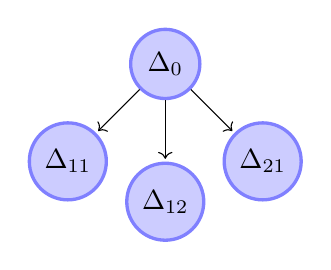
\begin{tikzpicture}[shorten >=1pt,node distance=1.75cm,on grid,
    every state/.style={draw=blue!50,very thick,fill=blue!20}]
  \tikzstyle{nodeG}=[circle,thick,draw=gray!75,fill=green!20,minimum size=10mm]
  \tikzstyle{nodeR}=[circle,thick,draw=gray!75,fill=red!20,minimum size=10mm]
  \tikzstyle{nodeB}=[circle,thick,draw=gray!75,fill=blue!20,minimum size=10mm]
  \tikzstyle{nodeI}=[state, circle,thick,draw=gray!75,fill=blue!20,minimum size=10mm]

  % Original nodes
  \node[nodeB, state]          (q_000)              {$\Delta_0$};
  \node[nodeB, state]          (q_111) [below right=of q_000] {$\Delta_{21}$};
  \node[nodeB, state]          (q_222) [below left=of q_000] {$\Delta_{11}$}; 
  \node[nodeB, state]          (q_333) [below = of q_000] {$\Delta_{12}$};

  \path[->] (q_000) edge node [above right] {} (q_111);
  \path[->] (q_000) edge node [above left]  {} (q_222);
  \path[->] (q_000) edge node [below]       {} (q_333);
\end{tikzpicture}
}
\caption{Under the eye of the monitor}
\label{fig:monitorpersp}
\end{figure}

If the context tree were structured as shown in \Cref{fig:monitorpersp}, then
the property $\varphi_2 = \Theta(\alpha_2 : \delta_2)$ would correctly target
the desired contexts. However, it is not feasible to construct a new context
tree each time such a need arises.

The creation of contexts is tied to the actual interactions occurring in the
system. For example, context $\Delta_1$ is generated in response to the
appearance of a specific message. Accordingly, we can visualize the context
tree such that transitions between nodes correspond to the messages that
triggered the creation of each context, as illustrated in
\Cref{fig:contextexample}.
 
\begin{figure}[ht]
\centering
\usetikzlibrary{arrows.meta, positioning, automata, shapes.geometric}
\scalebox{1}{%
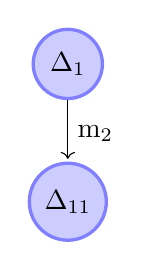
\begin{tikzpicture}[shorten >=1pt,node distance=1.75cm,on grid,
    every state/.style={draw=blue!50,very thick,fill=blue!20}]
  \tikzstyle{nodeG}=[circle,thick,draw=gray!75,fill=green!20,minimum size=10mm]
  \tikzstyle{nodeR}=[circle,thick,draw=gray!75,fill=red!20,minimum size=10mm]
  \tikzstyle{nodeB}=[circle,thick,draw=gray!75,fill=blue!20,minimum size=10mm]
  \tikzstyle{nodeI}=[state, circle,thick,draw=gray!75,fill=blue!20,minimum size=10mm]

  % Original nodes
  \node[nodeB, state]          (q_000)              {$\Delta_1$};
  \node[nodeB, state]          (q_111) [below =of q_000] {$\Delta_{11}$};

  \path[->] (q_000) edge node [below right, near start] {m$_2$} (q_111);
\end{tikzpicture}
}
\caption{Message pipelining into contexts}
\label{fig:contextexample}
\end{figure}

All of these messages remain part of the system, and their corresponding
contexts continue to be created. However, when our goal is to verify a property
specifically over the children of $\Delta_1$ and $\Delta_2$, it becomes
important to take into account the parent contexts and the messages that
triggered their creation.

To address this, WALTZ provides a mechanism to selectively “ignore” certain
contexts and focus only on the relevant ones, allowing us to specify the level
of the context tree on which to operate. For example, by defining the property
$\varphi_2$ as:
$$
\varphi_2 = \Theta( \ \Theta(\alpha_2 : \delta_2))
$$

we gain the ability to verify the property $\alpha_2 : \delta_2$ specifically
within the contexts $\Delta_{11}$, $\Delta_{12}$, and $\Delta_{21}$. Nesting
the $\Theta$ operator in this way effectively directs the evaluation to a
particular level of the context tree, while other contexts are ignored. These
ignored contexts remain part of the system’s logical structure, but they do not
influence the current verification, allowing the monitor to concentrate solely
on the relevant sub-traces.

This approach allows us to check whether at least one message from any client
satisfies $\delta_2$, even if a client fails to connect successfully, since we
are only interested in the ones that did connect with success. Similarly, if we
want to ensure that all messages from all clients satisfy $\delta_2$, we can
express this with a nested $\Omega$ operator, defining $\Omega( \
\Omega(\alpha_2 : \delta_2))$.

Returning to the property $\varphi_2 = \Theta( \ \Theta(\alpha_2 : \delta_2))$,
and the contexts shown in \Cref{fig:monitorinterpretation}. We can see that the
semantics correctly handle the evaluation, verifying the satisfaction of this
formula at the intended level of the context tree.

We begin by evaluating $\Theta(  \ \Theta(\alpha_2 : \delta_2))$, which
corresponds to the following semantic check:
$$
\sigma, \Delta_0 \;&\models\; \Theta( \ \Theta(\alpha_2 : \delta_2)) \text{ iff } \exists_{\Delta_{k} \blacktriangleright \Delta_0} : \sigma, \Delta_{k} \models \Theta(\alpha_2 : \delta_2)
$$

At this level, the outer $\Theta$ considers all contexts directly forked from
$\Delta_0$, which are $\Delta_1$ and $\Delta_2$. For each of these contexts, we
now evaluate the inner formula $\Theta(\alpha_2 : \delta_2)$.

Focusing first on $\Delta_1$, the inner $\Theta$ descends one level further to
examine its child contexts, verifying whether any of them satisfy $\alpha_2 :
\delta_2$. The same process is then applied to $\Delta_2$ and its children. In
this way, the nested structure of $\Theta$ ensures that the property is checked
at the appropriate level of the context tree while ignoring irrelevant
branches. The semantic check for $\Delta_1$ is: 
$$
\sigma, \Delta_1 \;&\models\; \Theta (\alpha : \delta) \text{ iff } \exists_{\Delta_{k} \blacktriangleright \Delta_1} : \sigma, \Delta_{k} \models (\alpha_2 : \delta_2)
$$

As we can observe, each time we unpack a modal operator, we descend one level
in the context tree, examining the children of the current context under
evaluation. This approach provides a powerful mechanism for focusing
specifically on a single level of messages entering the system. With this step
complete, the remaining verifications to be performed are:
\[
\begin{align*}
  \varphi_{11} = \sigma, \Delta_{11} \models (\alpha_2 : \delta_2) \\
  \varphi_{12} = \sigma, \Delta_{12} \models (\alpha_2 : \delta_2)
\end{align*}
\]

The same verification will be applied to $\Delta_2$. It is sufficient that at
least one message within the contexts $\Delta_{11}$, $\Delta_{12}$, or
$\Delta_{21}$ adheres to $\delta_2$. If none of these messages satisfy the
property, the monitor continues observing the system, issuing inconclusive
verdicts, as is typical in runtime monitoring.

In conclusion, this example illustrates how different ways of specifying
properties directly affect how the monitor interprets chains of messages. By
navigating the context tree, we can choose to evaluate properties across the
entire structure or focus on a specific level, as demonstrated in this section. This
flexibility effectively shifts the monitor’s perspective on the trace it
witnesses, allowing it to check properties in a manner aligned with the intended
system behaviour.

\section{The Compilation Process}
\label{sec:waltz_compilation}
At the core of WALTZ is the idea that high-level specifications can be
transformed into executable entities, running processes that continuously
observe a system and determine whether it behaves as intended. This active
component is referred to as the monitor, which, in our implementation, takes
the form of executable \texttt{Erlang} code.

We begin by examining the compilation pipeline, implemented in \texttt{OCaml}~\cite{ocaml}
for its strong type system and functional programming capabilities, which make
it well-suited for building a robust parser and compiler. The pipeline takes a
WALTZ formula, provided as a simple \texttt{.txt} file, parses it according to
our defined grammar, and translates it into optimized \texttt{Erlang} code
ready for execution. The generated monitor is then attached to the system and
runs alongside it, receiving relevant events to verify the defined properties.
The details of this attachment and instrumentation process are discussed in
\Cref{cha:actorchestra}.

To make this process more approachable (both for ourselves and for the tool),
we slightly adapted the formal grammar described in the previous section. The
semantics remain untouched, but we have introduced a few carefully chosen
“quality-of-life” tokens. These small adjustments make the parser’s job easier,
reduce the chance of errors, and allow the code generator to work more
smoothly, without compromising the expressiveness or rigor of WALTZ.

\iffalse
To introduce the topic, we begin with a simple example that will help clarify
the discussion. Consider the following WALTZ property:
\[
\varphi =
\Omega\left(
\begin{aligned}
 &\text{\texttt{send$_{\text{client} \rightarrow \text{server}}$}}\{\_, \text{\texttt{Number, Ref}}\} : \top\ ; \\
 &\quad\text{\texttt{send$_{\text{server} \rightarrow \text{client}}$}}\{\_, \text{\texttt{NumberReturn, Ref}}\} :
   \text{\texttt{NumberReturn = 2 * Number}}
\end{aligned}
\right)
\]

When fed into the compilation pipeline, this property produces the following
\texttt{Erlang} monitor, with some syntax missing due to presentation purposes:

\begin{erlang}[caption={Monitor example}, label={lst:monitorexample}]
  a():
    receive {client, server, Msg1, Context} ->
      case Msg1 of {_, Number, Ref} ->
        receive {server, client, Msg2, Context} ->
          case Msg2 of {_, Result, Ref} ->
            if (Result == Number * 2) -> a()
            true -> io:format("Property Violated")
          ... 
\end{erlang}
\fi
\subsection{Practical Grammar Changes}
\label{sub_sec:practical_grammar}

In order to ease our parsing and compilation job, we add some useful tokens into
our grammar. The new WALTZ grammar will be defined as:

\begin{definition}[WALTZ Formula]
  The set of WALTZ formulas is defined by the following grammar:
\end{definition}
\[
\begin{align*}
\varphi \;&::=\; 
  \text{\texttt{OMEGA}} (\varphi) \;|\; \text{\texttt{THETA}} (\varphi) \;|\; \varphi \ ; \ \varphi  \;|\; \alpha : \delta \\  
\delta \;&::=\; \top \;|\; \bot \;|\; c \;|\; \lnot \delta \\ 
  \alpha \;&::=\; \texttt{send}_{\texttt{id} \rightarrow \texttt{id}} \ \texttt{WITH} \ \{  \texttt{M} \} \\
\texttt{M} \;&::=\; \texttt{T} \;|\; \texttt{T} \; , \texttt{M} \;|\; \{ \texttt{M} \}  \\
  \texttt{T} \;&::=\; (\texttt{cons} \;|\; \texttt{var}) \\
\end{align*}
\]

During this section we still might use the mathematical symbols of $\Omega$ and
$\Theta$, but have in mind that the specification files themselves, will work
with the keyword \texttt{OMEGA} and \texttt{THETA}. Another useful addition is
the \texttt{WITH} keyword, that is present in the signatures of the messages,
separating the \texttt{send} request origin and destination from the signature
of the message itself. More on this, can be consulted in the
\href{https://github.com/vladbug/ACTORCHESTRA.git}{\texttt{ACTORCHESTRA}} page,
which has a comprehensive list of property definitions, and the full grammar
for property specifications.

\subsection{The General Monitor Structure}
\label{sub_sec:general_mon_struct}
The design of our monitors is essential to ensure adherence to the rules we
defined for property verification. A central concept in this design is the
notion of context, which is critical to understanding how the monitor processes
incoming traces from the system.

To simulate the consumption of contexts and message chains, the monitor
compilation is implemented as a sequence of \texttt{receive} statements. These
statements serve as the primary mechanism for capturing messages not only in
the correct order of the chain but also within their respective contexts, as
illustrated in Listing \ref{lst:messagechain}.

\begin{lstlisting}[float=htbp, language=erlang, caption=Message Chains, label={lst:messagechain}]
    receive Signature1 ->
      if BooleanConstraint1 ->
        receive Signature2 ->
          if BooleanConstraint2 ->
            ... 
\end{lstlisting}

As the monitor consumes a message chain, it progresses sequentially through the
\texttt{receive} statements, checking property satisfaction at each step. Once
the entire chain has been processed, the monitor either loops back to handle
the next chain or produces a verdict, depending on the property being
monitored. This architecture not only enforces the order and unbreakability of
messages but also preserves the context in which each event is evaluated and
maintains the scope of all variables involved in the interaction.

Take for example the property
$\Omega(\text{\texttt{send$_{\text{\texttt{actorA}} \rightarrow
\text{\texttt{actorB}}}$}} \{\text{\texttt{MyPID, Payload}}\} :
\{\text{\texttt{Payload}}\} > 0)$, which checks if the property is satisfied
across all contexts. The monitor for this property can be visualized in Listing
\ref{lst:omegamon}

\begin{lstlisting}[float=htbp, language=erlang, caption=\text{$\Omega$} monitor example, label={lst:omegamon}]
loop():
  receive {actorA, actorB, Msg, Context} ->
    case Msg1 of {MyPid, Payload} ->
      if (Payload > 0) -> loop()
      true -> io:format("(*@$\text{\ding{56}}$@*)")
      end;
    end;
  end;
end.
\end{lstlisting}

Since this property is encapsulated within an $\Omega$, the monitor focuses on
detecting violations. If the current message chain satisfies the property, the
monitor simply invokes \texttt{loop()} to evaluate the next chain. If the
property is not satisfied, a violation is reported. Each call to
\texttt{loop()} prepares the monitor to verify the property against a new
context.

\iffalse
To illustrate this more concretely, consider the context tree shown in
\Cref{fig:contextformonitor}. The verification of the property for each context
corresponds to three recursive calls to the monitor’s \texttt{loop()} function.
Each call processes a single context and evaluates the property within it,
following the same principles defined in the WALTZ semantics. 

\begin{figure}[ht]
\centering
\usetikzlibrary{arrows.meta, positioning, automata, shapes.geometric}
\scalebox{1}{%
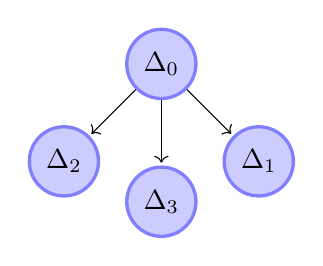
\begin{tikzpicture}[shorten >=1pt,node distance=1.75cm,on grid,
    every state/.style={draw=blue!50,very thick,fill=blue!20}]
  \tikzstyle{nodeG}=[circle,thick,draw=gray!75,fill=green!20,minimum size=10mm]
  \tikzstyle{nodeR}=[circle,thick,draw=gray!75,fill=red!20,minimum size=10mm]
  \tikzstyle{nodeB}=[circle,thick,draw=gray!75,fill=blue!20,minimum size=10mm]
  \tikzstyle{nodeI}=[state, circle,thick,draw=gray!75,fill=blue!20,minimum size=10mm]

  % Original nodes
  \node[nodeB, state]          (q_000)              {$\Delta_0$};
  \node[nodeB, state]          (q_111) [below right=of q_000] {$\Delta_{1}$};
  \node[nodeB, state]          (q_222) [below left=of q_000] {$\Delta_{2}$}; 
  \node[nodeB, state]          (q_333) [below = of q_000] {$\Delta_{3}$};

  \path[->] (q_000) edge node [above right] {} (q_111);
  \path[->] (q_000) edge node [above left]  {} (q_222);
  \path[->] (q_000) edge node [below]       {} (q_333);
\end{tikzpicture}
}
\caption{Context tree example}
\label{fig:contextformonitor}
\end{figure}
\fi

For the $\Theta$ operator, the overall structure of the monitor remains the
same as before, with message chains captured in the same manner as shown in
Listing \ref{lst:messagechain}. The key differences lie in the evaluation
strategy and the stopping condition: rather than seeking violations, the
monitor now continues processing messages until it finds a chain that satisfies
the property. Once such a chain is detected, the property is considered
satisfied, and the corresponding verdict is produced. As an example, the
compiled monitor for the property
$\Theta(\text{\texttt{send$_{\text{\texttt{actorA}} \rightarrow
\text{\texttt{actorB}}}$}} \{\text{\texttt{MyPID, Payload}}\} :
\{\text{\texttt{Payload}}\} > 0)$ is shown in Listing
\ref{lst:monitortheta}.

\begin{lstlisting}[float=htbp, language=erlang, caption=\text{$\Theta$} monitor example, label={lst:monitortheta}]
loop():
  receive {actorA, actorB, Msg, Context} ->
    case Msg1 of {MyPid, Payload} ->
      if (Payload > 0) -> io:format("(*@$\text{\ding{52}}$@*)")
      true -> loop() 
      end;
    end;
  end;
end.
\end{lstlisting}

As we can see, the \texttt{Erlang} abstraction and design techniques make the 
transition of WALTZ semantics, into simple yet robust monitor executables
that are able to capture these messages at runtime. 
\subsection{The Preservation of Context}
\label{sub_sec:context_preservation}
The monitor expects to receive the following tuple at runtime:
$$
\text{\texttt{\{Sender, Receiver, Message, Context\}}}
$$

We will see in the next chapter how this is achieved, but for now, consider
this as the signature produced by \texttt{Erlang}’s internal tracing
mechanisms. It is important to note that, while the context appears as part of
the message payload, the system itself is not required to explicitly include it
in the messages. As we will explore in the next chapter, it is possible to
build correct \texttt{Erlang} systems without manually managing the causality
of messages by leveraging the OTP behaviour discussed previously in
\Cref{sec:OTP}.

A natural question arises: how can we ensure that the monitor observes only the
messages belonging to a specific chain? This is precisely where the context
plays a crucial role. Consider the property $\varphi$:
$$
\varphi = \Theta(\text{\texttt{send$_{\text{\texttt{actorA}} \rightarrow
\text{\texttt{actorB}}}$}} \ \{\text{\texttt{MyPID, X, Y}}\} : \top \ ; \ \text{\texttt{send$_{\text{\texttt{actorB}} \rightarrow
\text{\texttt{actorC}}}$}} \ \{\text{\texttt{MyPID2, Z}}\} : \text{\texttt{Z = X + Y}})
$$

The goal is to verify that at least one context, a chain of causally related
messages, satisfies the defined property. Without proper context management, the
monitor could mistakenly associate messages, as concurrent \texttt{Erlang}
processes can produce events in many possible orders. For example, consider the
following trace:
\[
\begin{align*}
  \text{\texttt{m$_1$}} \;&=\; \text{\texttt{send$_{\text{\texttt{actorA}} \rightarrow
\text{\texttt{actorB}}}$}} \ \{\text{\texttt{actorA, 10, 10}}\}  \\
  \text{\texttt{m$_2$}} \;&=\; \text{\texttt{send$_{\text{\texttt{actorA}} \rightarrow
\text{\texttt{actorB}}}$}} \ \{\text{\texttt{actorA, 20, 10}}\} \\
  \text{\texttt{m$_3$}} \;&=\; \text{\texttt{send$_{\text{\texttt{actorB}} \rightarrow
\text{\texttt{actorC}}}$}} \ \{\text{\texttt{actorB, 30}}\} \\
  \text{\texttt{m$_4$}} \;&=\; \text{\texttt{send$_{\text{\texttt{actorB}} \rightarrow
\text{\texttt{actorC}}}$}} \ \{\text{\texttt{actorB, 20}}\} 
\end{align*}
\]

The monitor generated from $\varphi$ is presented in Listing \ref{lst:monitornocontext}. 

\begin{erlang}[caption={Wrong Monitor for $\varphi$}, label={lst:monitornocontext}]
loop():
  receive {actorA, actorB, Msg1} ->
    case Msg1 of {MyPid, X, Y} ->
      receive {actorB, actorC, Msg2} ->
        case Msg2 of {MyPid2, Z} ->
          if (Z == X + Y) -> io:format("(*@$\text{\ding{52}}$@*)")
          true -> loop()
          ...
\end{erlang}

Without context awareness, it is insufficient to assume that the monitor will
read messages from each context in the order the events occurred. While
\texttt{Erlang} guarantees message ordering between two processes, this
guarantee does not extend across multiple processes. Consequently, the monitor
may encounter various interleavings of messages, such as the following:
\[
\begin{align*}
\text{\texttt{m$_1$}} \ \text{\texttt{m$_4$}} \ \text{\texttt{m$_2$}} \ \text{\texttt{m$_3$}} \\
\text{\texttt{m$_2$}} \ \text{\texttt{m$_3$}} \ \text{\texttt{m$_1$}} \ \text{\texttt{m$_4$}} \\
\text{\texttt{m$_2$}} \ \text{\texttt{m$_1$}} \ \text{\texttt{m$_4$}} \ \text{\texttt{m$_3$}} \\
\text{\texttt{m$_2$}} \ \text{\texttt{m$_1$}} \ \text{\texttt{m$_3$}} \ \text{\texttt{m$_4$}}
\end{align*}
\]

These are all valid interleavings that the monitor might observe, and in some
cases, values from one causal chain, such as \texttt{X} and \texttt{Y}, could
be incorrectly combined with \texttt{Z} from another chain. This is highly
problematic, as it can lead to erroneous verdicts for the properties being
monitored.

For example, suppose the monitor first captures message \texttt{m$_1$}, and
then, due to a possible interleaving, observes \texttt{m$_2$} followed by
\texttt{m$_3$}. In the code shown in Listing \ref{lst:monitornocontext},
\texttt{m$_1$} matches the first \texttt{receive} clause, assigning the runtime
values \texttt{10} to both \texttt{X} and \texttt{Y}. When \texttt{m$_2$}
arrives, it does not match the second \texttt{receive} clause for the chain and
remains in the mailbox. Subsequently, \texttt{m$_3$} matches its expected
signature, assigning \texttt{30} to \texttt{Z}. The verification of \texttt{Z
== X + Y} then fails, since \texttt{10 + 10} $\neq$ \texttt{30}.

Then, the monitor might match \texttt{m$_2$} followed by
\texttt{m$_4$}, which do not belong to the same causal chain. This again can
result in a property violation, even though, in reality, the property was
was satisfied in both contexts.

This illustrates why attaching context to messages is absolutely crucial. With
context information, the monitor can use pattern matching to “lock” onto a
specific chain: once the first message matches the start of a \texttt{receive}
chain, only messages belonging to the same context are accepted. Messages from
other contexts may still arrive in the monitor’s mailbox, but they will wait
until the current chain has been fully processed.
\subsection{Non Breakable Chains}
\label{sub_sec:waltz_nonbreak}
As discussed in previous sections, message chains are unbreakable. By
structuring the monitors as nested \texttt{receive} clauses and leveraging the
context of each message, the monitor can process messages chain by chain,
ensuring that payloads from different contexts are never mixed. If any message
within a chain violates its boolean constraint, the monitor’s next action
depends on the type of property being monitored: it will either proceed to the
next chain or immediately report a property violation. For instance, consider
the following property:
$$
\alpha_1 : \delta_1 \ ; \ \alpha_2 : \delta_2 \ ; \ \alpha_3 : \delta_3
$$

In the generated monitor code, there are three nested \texttt{receive} clauses,
as shown in Listing \ref{lst:monitornesting}. To simplify the presentation of
our monitors, we will use a combination of mathematical notation and pseudocode
instead of strictly syntactically correct \texttt{Erlang} code. The behaviour
of the monitor depends on the chosen modal operator. When monitoring the
property $\Omega(\alpha_1 : \delta_1 \ ; \ \alpha_2 : \delta_2 \ ; \ \alpha_3 :
\delta_3)$, a single broken message chain is sufficient to declare the property
violated. In contrast, for the property  $\Theta(\alpha_1 : \delta_1 \ ; \
\alpha_2 : \delta_2 \ ; \ \alpha_3 : \delta_3)$  the property is considered
satisfied as soon as there exists one context in which the entire chain remains
unbroken.

\begin{erlangmin}[caption={Nesting receive clauses}, label={lst:monitornesting}]
  loop():
    receive (*@$\alpha_1$@*) ->
      check (*@$\delta_1$@*) ->
        receive (*@$\alpha_2$@*) ->
          check (*@$\delta_2$@*) ->
            receive (*@$\alpha_3$@*) ->
              check (*@$\delta_3$@*) ->
\end{erlangmin}

\iffalse
\begin{erlangmin}[caption={$\Omega$ behaviour with chains}, label={lst:monitornestomega}]
  loop():
    receive (*@$\alpha_1$@*) ->
      check (*@$\delta_1$@*) -> 
        if(!(*@$\delta_1$@*)) then (*@$\text{\ding{56}}$@*)  
        receive (*@$\alpha_2$@*) ->
          check (*@$\delta_2$@*) ->
            if(!(*@$\delta_2$@*)) then (*@$\text{\ding{56}}$@*) 
            receive (*@$\alpha_3$@*) ->
              check (*@$\delta_3$@*) ->
                if(!(*@$\delta_3$@*)) then (*@$\text{\ding{56}}$@*) 
                else loop()
\end{erlangmin}

As we can see in Listing \ref{lst:monitornestomega}, each time we will perform the
check of the boolean constraints associated with each message, it is sufficent for
one to fail to the entire property to be violated. If everything goes like it should, then
we will continue monitoring the property by re-entering the \texttt{loop()} recursively.

The tricky part comes right now, if we monitor for $\Theta(\alpha_1 : \delta_1 \ ; \
\alpha_2 : \delta_2 \ ; \ \alpha_3 : \delta_3)$, even if there is a failure, we
want to reset the whole verification to begin receiving another chain. A problem comes
with this though, if $\alpha_1$ fails to adhere to $\delta_1$, we cannot immediately jump
to the beginning of the receive chain, because $\alpha_2$ and $\alpha_3$ will be 
stuck in the mailbox, and that might cause problems in terms of overhead, since they
will be always checked in order to see if they match any \texttt{receive}, but it also
provides some logical problems that might happen.

As we will see in \Cref{cha:actorchestra}, we might have systems where the context
that is attached to the messages, among the same client, will be always the same, and 
with that, two different client interactions will actually have the same context, even though
to the eyes of the monitor they will be different, because we will process them 
separately. By leaving "dead" messages in the mailbox of the monitor, we risk to
match them when then same client performs a request again but with a different intent. We
will see that this is a problem in some systems, not in all.

Therefore, in order to solve both problems, what will happen is that when a chain is
broken, we still consume the whole chain of that context from the mailbox, but we will 
have a special flag, which will tell us at the end of processing the entire chain, whether
at some point it was broken or not, as depicted in Listing \ref{lst:monitornesttheta}.

With this approach, we will clean the mailbox from messages that belong to a
chain that has already been broken, because they will now become irrelevant,
but we still want to consume them from the mailbox, to remove unnecessary
constant checking, and avoid possible logical errors in the future of the
trace.

\begin{erlangmin}[caption={$\Theta$ behaviour with chains}, label={lst:monitornesttheta}]
  loop():
    receive (*@$\alpha_1$@*) ->
      check (*@$\delta_1$@*) -> 
        if(!(*@$\delta_1$@*)) then flag
        receive (*@$\alpha_2$@*) ->
          check (*@$\delta_2$@*) ->
            if(!(*@$\delta_2$@*)) then flag
            receive (*@$\alpha_3$@*) ->
              check (*@$\delta_3$@*) ->
                if(!(*@$\delta_3$@*)) then flag
                if(flag) loop()
                else (*@$\text{\ding{52}}$@*) 
\end{erlangmin}

There is an issue though, for bigger chains, will slow down the performance of
our monitor, because before processing one chain, he has to finish the current
one. In practice, no property would realistically have 100 chained messages,
but if that were the case, then we would slow down, not the system, but the
monitor perception of what the system is doing, as if it stops in time compared
to the real events happening in the system. 

We would like to have the monitor to trully run alongside the system, and
capture all the messages as they indeed happen, which with the current
structure works, but when messages are in the monitor's mailbox, that means
that they already occurred and if a violation is indeed detected, we would only
capture that once it goes through the monitor. We will see in the section of
optimizations, what is possible to do in order to fix this "stuck in time"
issue.
\fi
\subsection{Compilation of $\Omega$}
\label{sub_sec:waltz_omega_comp}

As discussed previously, the $\Omega$ operator allows us to define a monitor
that verifies whether a property holds in every context of the system; if any
context fails, the property is considered violated. In general, we can define
properties of increasing complexity, such as:
\[
\begin{align*}
  \varphi_1 \;&=\; \Omega(\alpha : \delta) \\
  \varphi_2 \;&=\; \Omega(\alpha_1 : \delta_1 \ ; \ \alpha_2 : \delta_2) \\
  \varphi_3 \;&=\; \Omega(\alpha_1 : \delta_1 \ ; \ \alpha_2 : \delta_2 \ ; \ \alpha_3 : \delta_3)
\end{align*}
\]

To keep the discussion focused, we will set aside the nesting of modal
operators for now, as they introduce additional complexity that we will address
in a later section. In this compilation showcase, we concentrate on compiling
monitors for single message chains without nested operators. Using this
approach, the property $\varphi_2$ can be compiled into the \texttt{Erlang}
monitor shown in Listing \ref{lst:multipleomega}, which illustrates how
multiple sequential messages within a single chain are handled.

\begin{erlangmin}[caption={$\Omega$ monitor generation}, label={lst:multipleomega}]
  monitor_(*@$\varphi_2$@*)():
    receive (*@$\alpha_1$@*) ->
      check (*@$\delta_1$@*) -> 
        if(!(*@$\delta_1$@*)) then (*@$\text{\ding{56}}$@*)  
        receive (*@$\alpha_2$@*) ->
          check (*@$\delta_2$@*) ->
            if(!(*@$\delta_2$@*)) then (*@$\text{\ding{56}}$@*) 
            else monitor_(*@$\varphi_2$@*)() 
\end{erlangmin}

Each chain is going to be evaluated separately, flowing through the nested
chain of \texttt{receive} statements, at each moment doing a sanity check to
discover whether the property is being violated at that point or not.
Considering property $\varphi_2$, and the trace $\sigma =
\textcolor{blue}{\texttt{m$_1$}}^{\text{\ding{52}}} \
\textcolor{red}{\texttt{m$_2$}}^{\text{\ding{52}}} \
\textcolor{blue}{\texttt{m$_3$}}^{\text{\ding{56}}} \
\textcolor{red}{\texttt{m$_4$}}^{\text{\ding{52}}} ... $, with the boolean
constraints satisfactions indicated above it. Messages \texttt{m$_1$} and
\texttt{m$_2$} share the signature $\alpha_1$, while \texttt{m$_3$} and
\texttt{m$_4$} have signature $\alpha_2$. In this scenario, the monitor
processes each chain individually, ensuring that the property is evaluated
correctly for each sequence of causally related messages, as illustrated in
\Cref{fig:waltz_monitorwitness}.

\begin{figure}[ht]
\centering
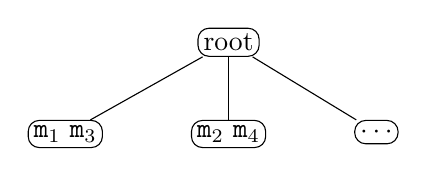
\begin{tikzpicture}[node distance=0.8cm and 1.2cm, every node/.style={draw, rounded corners, inner sep=2pt}]
    % Top node
    \node (oracle) {root};
    % Bottom-left node
    \node (leftab) [below left=of oracle] {\texttt{m$_1$} \texttt{m$_3$}};
    % Bottom-right node
    \node (middletab) [below =of oracle] {\texttt{m$_2$} \texttt{m$_4$}};
    % Bottom-right node
    \node (rightab) [below right=of oracle] {$\cdots$};

    % Edges
    \draw (oracle) -- (leftab);
    \draw (oracle) -- (rightab);
    \draw (oracle) -- (middletab);
\end{tikzpicture}
\caption{The monitor message flow for property $\varphi_2$}
\label{fig:waltz_monitorwitness}
\end{figure}

Each message in a chain is evaluated within its designated context, ensuring
that it is checked against the specified property in the correct scope.

\iffalse
Each “bubble” can be seen as a distinct path through the monitor’s
\texttt{receive} chain. When the monitor loops back to process the next chain,
it effectively transitions from one path to another, systematically verifying
all possible sequences of causally related messages.
\fi
\subsection{Compilation of $\Theta$}
\label{sub_sec:waltz_theta_comp}
The $\Theta$ operator allows verification of whether at least one context in
the system satisfies a given property. Once any context meets the required
condition, the property can be considered satisfied, enabling the monitor to
halt further evaluation. This operator thus allows the definition of
properties such as:
\[
\begin{align*}
  \varphi_1 \;&=\; \Theta(\alpha : \delta) \\
  \varphi_2 \;&=\; \Theta(\alpha_1 : \delta_1 \ ; \ \alpha_2 : \delta_2) \\
  \varphi_3 \;&=\; \Theta(\alpha_1 : \delta_1 \ ; \ \alpha_2 : \delta_2 \ ; \ \alpha_3 : \delta_3)
\end{align*}
\]

The monitor generated from property $\varphi_3$ is present in Listing \ref{lst:thetagen}. 

\begin{erlangmin}[caption={$\Theta$ behaviour with chains}, label={lst:thetagen}] 
  monitor_(*@$\varphi_3$@*)():
    receive (*@$\alpha_1$@*) ->
      check (*@$\delta_1$@*) -> 
        if(!(*@$\delta_1$@*)) then flag
        receive (*@$\alpha_2$@*) ->
          check (*@$\delta_2$@*) ->
            if(!(*@$\delta_2$@*)) then flag
            receive (*@$\alpha_3$@*) ->
              check (*@$\delta_3$@*) ->
                if(!(*@$\delta_3$@*)) then flag
                if(flag) then monitor_(*@$\varphi_3$@*)()
                else (*@$\text{\ding{52}}$@*) 
\end{erlangmin}

We can observe that the overall pattern remains consistent: as chains grow
longer, additional nested clauses are introduced to represent the extended
sequence of messages. This structuring allows the monitor to traverse each
chain and determine whether there exists at least one chain in which all
messages satisfy their respective boolean constraints.

The \texttt{flag} is essential for detecting when a chain has been broken. It
ensures that once a chain is invalidated, the monitor can correctly consume the
remaining messages without mistakenly treating them as contributing to property
satisfaction. Without this mechanism, such as in the monitor generated in
Listing \ref{lst:thetagenwrong}, several potential errors could occur.

\begin{erlangmin}[caption={$\Theta$ problematic monitor}, label={lst:thetagenwrong}] 
  monitor_(*@$\varphi_3$@*)():
    receive (*@$\alpha_1$@*) ->
      check (*@$\delta_1$@*) -> 
        if(!(*@$\delta_1$@*)) then monitor_(*@$\varphi_3$@*)() 
        receive (*@$\alpha_2$@*) ->
          check (*@$\delta_2$@*) ->
            if(!(*@$\delta_2$@*)) then monitor_(*@$\varphi_3$@*)()
            receive (*@$\alpha_3$@*) ->
              check (*@$\delta_3$@*) ->
                if(!(*@$\delta_3$@*)) then monitor_(*@$\varphi_3$@*)()
                else (*@$\text{\ding{52}}$@*) 
\end{erlangmin}

Consider a scenario in which, for a given trace, the message matching
$\alpha_1$ fails to satisfy the boolean constraint $\delta_1$. If we were to
simply make a recursive call the subsequent messages of that interaction chain
would remain in the mailbox. Repeating this process multiple times could result
in the mailbox being filled with “garbage” messages.

The issue becomes particularly critical in systems where an entire client
session is treated as a single causal chain. In these cases, multiple messages
may belong to the same context, as discussed in \Cref{cha:actorchestra}, and
failing to properly discard broken or invalid messages from the mailbox can
result in inconsistencies.

By following this architecture for compiling the $\Theta$ operator, we not only
prevent the accumulation of irrelevant messages but also safeguard against
potential inconsistencies caused by leftover messages in the mailbox.
\section{Compilation of Nested Modal Operators}
\label{sec:waltz_nested_comp}

It is also necessary to address the compilation of nested operators, as well as
the structure of the monitors that result from such properties. Compared to the
cases introduced earlier, these monitors exhibit higher complexity, but this
complexity is essential: it allows us to analyse behavioural patterns that go
beyond the verification of simple message chains defined by a single modal
operator. Nesting enables properties to capture relationships across multiple
levels of causality, reflecting scenarios where interactions are hierarchically
dependent. To illustrate this idea, let us start by considering the following property:
$$
\varphi_1 = \Theta(\alpha_1 : \delta_1 \ ; \ \Theta(\alpha_2 : \delta_2))
$$

Recalling the example and the concepts presented in \Cref{sec:waltz_nesting}
and \Cref{sec:waltz_monitor_interpretation}, we treat the messages within each
context as finite chains. Nesting extends this model by introducing a hierarchy
and explicit relationships between contexts, allowing child contexts to inherit
causal dependencies from their parents and enabling the monitor to correctly
evaluate message chains across multiple levels. This extension allows us to
capture dependencies between chains that belong to the same parent context. A
representative example is the interaction where a client connects to the
system, establishing the initial context, and subsequently issues multiple
requests. Each request corresponds to a distinct event, yet all of them remain
causally linked to the client’s initial connection.

The monitor generated for $\varphi_1$ is shown in Listing
\ref{lst:nestedtheta}. The fundamental idea here is the introduction of
sub-monitors. Rather than relying on a single monitor, the system now maintains
multiple monitors, one for each parent context. The central oracle,
corresponding to $\Delta_0$, assumes the responsibility of routing messages to
the appropriate sub-monitor. Each sub-monitor then independently evaluates its
portion of the property and reports back to its parent context whenever a
satisfaction or violation is detected.

\begin{erlangmin}[caption={$\Theta$ operator monitor nesting}, label={lst:nestedtheta}]
monitor_(*@$\varphi_1$@*)():
  receive 
    {Src, Dst, Msg, Context} ->
      if has_sub_monitor(Context) 
        route({Src, Dst, Msg, Context})
      else main_monitor({Src, Dst, Msg, Context})

main_monitor({Src, Dst, Msg, Context}):
  case {Src, Dst, Msg} of 
    (*@$\alpha_1$@*) ->
      check (*@$\delta_1$@*) ->   
        if(!(*@$\delta_1$@*)) then flag
        if(flag) then monitor_(*@$\varphi_1$@*)
        else
          spawn(sub_monitor_loop(), (*@$\Delta_{\text{\texttt{current}}}$@*), env),
          monitor_(*@$\varphi_1$@*)()
%sub_monitor_loop().erl 
sub_monitor_loop():
  receive (*@$\alpha_2$@*) ->
    check (*@$\delta_2$@*) ->
      if(!(*@$\delta_2$@*)) then flag
      if(flag) then sub_monitor_loop()
      else ping(monitor_(*@$\varphi_1$@*), (*@$\text{\ding{52}}$@*))  
\end{erlangmin}

As illustrated in Listing \ref{lst:nestedtheta}, the monitor now spawns an
additional process responsible for handling the child contexts derived from a
parent. This sub-monitor follows the same general structure we have already
seen for the compilation of $\Omega$ and $\Theta$, but with one important
difference: whenever it reaches a verdict, it must communicate this outcome
back to the monitor that created it. This is achieved through a simple
\texttt{ping} mechanism, enabling the parent to aggregate the results of its
children and decide its own verdict.

A crucial detail here is that, besides inheriting the context upon which the
child is spawned, denoted as $\Delta_{\text{\texttt{current}}}$, the
sub-monitor must also inherit the current \texttt{environment}. This ensures
that any variable bindings established at the parent level remain available to
the child monitors. Such sharing is essential because contexts, while evaluated
independently, are still hierarchically related: together they form causal
chains of events. By propagating both the context and the variable environment,
we preserve the ability to reason consistently across parent–child relations,
ensuring correctness when evaluating properties that depend on shared values.

It is also possible to nest $\Omega$ operators, though generating monitors for
such properties is nontrivial. For instance, consider a property similar to
$\varphi_1$, but expressed using the $\Omega$ operator, denoted as $\varphi_2$.
$$
\varphi_2 = \Omega(\alpha_1 : \delta_1 \ ; \ \Omega(\alpha_2 : \delta_2))
$$

What this property aims to capture is whether, for all contexts derived from
$\Delta_0$, namely $\Delta_1$ and $\Delta_2$, every one of their child contexts
satisfies the condition $\delta_2$. Intuitively, this can be read as: for every
client connection, all subsequent requests must carry positive numbers. The
monitor generated for this property is presented in Listing
\ref{lst:nestedomega}.

\begin{erlangmin}[caption={$\Omega$ operator monitor nesting}, label={lst:nestedomega}]
monitor_(*@$\varphi_2$@*)():
  receive 
    {Src, Dst, Msg, Context} ->
      if has_sub_monitor(Context) 
        route({Src, Dst, Msg, Context})
      else main_monitor({Src, Dst, Msg, Context})

main_monitor({Src, Dst, Msg, Context}):
  case {Src, Dst, Msg} of 
    (*@$\alpha_1$@*) ->
      check (*@$\delta_1$@*) ->   
        if(!(*@$\delta_1$@*)) then (*@$\text{\ding{56}}$@*)
        else
          spawn(sub_monitor_loop(), (*@$\Delta_{\text{\texttt{current}}}$@*), env),
          monitor_(*@$\varphi_2$@*)()
%sub_monitor_loop().erl 
sub_monitor_loop():
  receive (*@$\alpha_2$@*) ->
    check (*@$\delta_2$@*) ->
      if(!(*@$\delta_2$@*)) then ping(monitor_(*@$\varphi_2$@*), (*@$\text{\ding{56}}$@*)) 
      else sub_monitor_loop() 
\end{erlangmin}

This structuring allows us to faithfully reproduce the context hierarchies
explored in the examples of the previous sections. For a complete generated
\texttt{Erlang} monitor, see \Cref{sec:waltz_monitor_example}. Additional
monitors and code examples can be found in the
\href{https://github.com/vladbug/ACTORCHESTRA.git}{online repository}.

\iffalse
One might still think, how do we compile properties like the one we have seen
in \Cref{sec:waltz_monitor_interpretation}, where there exists properties like
$\Omega( \Omega(\alpha : \delta) )$? Well, it is rather simple, and can be seen
in Listing \ref{lst:nestedomega2}.

\begin{erlangmin}[caption={$\Omega$ operand monitor nesting}, label={lst:nestedomega2}]
  monitor_(*@$\varphi_2$@*)():
    spawn(sub_monitor_loop(), (*@$\Delta_{\text{\texttt{current}}}$@*), env),
    monitor_(*@$\varphi_2$@*)()

  %sub_monitor_loop().erl 
  sub_monitor_loop():
    receive (*@$\alpha_2$@*) ->
      check (*@$\delta_2$@*) ->
        if(!(*@$\delta_2$@*)) then ping(monitor_(*@$\varphi_2$@*), (*@$\text{\ding{56}}$@*)) 
        else sub_monitor_loop()      
\end{erlangmin}

There will not be any type of property verification, and we will immediately
\texttt{spawn} the monitor responsible for the property checking. We will see
in \Cref{sec:waltz_optimizations} how we can transform this code in order to
avoid unnecessary monitor spawning.
\fi

\subsection{Compilation of Different Nested Modal Operators}
\label{sub_sec:waltz_nestednonmon}
In WALTZ, as we have seen it is possible to define properties with nested modal operators. This
greatly expands the expressiveness of the language but simultaneously opens the
Pandora’s box of non-monitorable properties. By the very nature of runtime
verification, combining different quantifiers, such as $\forall$ and $\exists$,
or in our case $\Omega$ and $\Theta$, can lead to monitors that will never be
able to produce a verdict during execution. To avoid such infinitely running
monitors, WALTZ explicitly alerts the user whenever a given property is
non-monitorable. This issue will be addressed in more detail in
\Cref{sec:waltz_monitorability}.

It is not difficult to see why such properties are problematic at runtime, even
if they may be meaningful from a specification standpoint. Consider, for
example, a property stating that “for every client, after a successful
connection, at least one of the subsequent requests carries a positive number.”
The monitor that would be generated for this property, which in WALTZ can be
written as $\varphi_3 = \Omega(\alpha_1 : \delta_1 \ ; \ \Theta(\alpha_2 :
\delta_2))$  would result in the structure shown in Listing
\ref{lst:nestednonmon}. 

\begin{erlangmin}[caption={Non monitorable property}, label={lst:nestednonmon}]
...
main_monitor({Src, Dst, Msg, Context}):
  case {Src, Dst, Msg} of 
    (*@$\alpha_1$@*) ->
      check (*@$\delta_1$@*) ->   
        if(!(*@$\delta_1$@*)) then (*@$\text{\ding{56}}$@*)
        else
          spawn(sub_monitor_loop(), (*@$\Delta_{\text{\texttt{current}}}$@*), env),
          monitor_(*@$\varphi_2$@*)()
%sub_monitor_loop().erl 
sub_monitor_loop():
  receive (*@$\alpha_2$@*) ->
    check (*@$\delta_2$@*) ->
      if(!(*@$\delta_2$@*)) then ping(monitor_(*@$\varphi_2$@*), (*@$\text{\ding{52}}$@*)) 
      else sub_monitor_loop()      
\end{erlangmin}

In this case, we can never reach a conclusive verdict. Assuming all client
connections are successful, the monitor will be forced to wait indefinitely: it
cannot guarantee that for every client the property will hold. It might hold
for some, or it might eventually be violated, but the monitor remains trapped
in uncertainty. The problem lies in the mismatch between parent and child
monitors, while the parent monitor expects a \texttt{ping} to signal a
violation, the child monitors only notify their parent upon satisfaction. As a
result, no definitive verdict is ever produced, and the monitor remains
inconclusive.

\iffalse
\section{Monitors Mailbox}
\label{sec:waltz_monitor_mailbox}
In order to understand how our monitors evaluate the messages in incoming trace, it is
crucial to understand the \texttt{Erlang} mailbox system. The monitor, or the monitors
in the case of nested properties, will receive the relevant events and process them 
accordingly. We have no guarantees in the order which they are received by the monitor,
since we are working with asynchronous systems, therefore it raises the need to have
the context associated to each message.

With the context being associated to each tuple, we are able to ignore certain messages
an leave them be in the mailbox, which will be processed in the future. Let us again
consider \Cref{ex:by2system}, our monitor could receive the following messages and
the mailbox would be structured like the one in \Cref{fig:stack}.

\begin{figure}[h!]
\centering
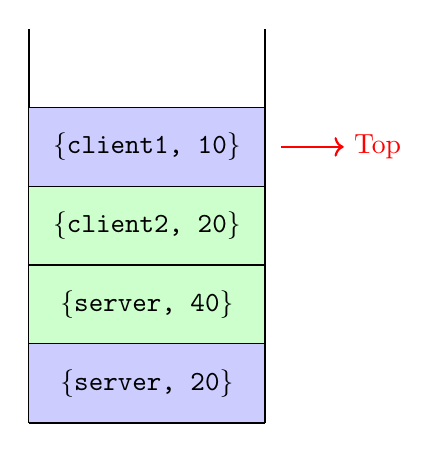
\begin{tikzpicture}
    % Draw stack container
    \draw[thick] (0,0) -- (0,5);  % left side
    \draw[thick] (3,0) -- (3,5);  % right side
    \draw[thick] (0,0) -- (3,0);  % bottom
    
    % Stack items
    \draw[fill=blue!20] (0,0) rectangle (3,1) node[midway]{\texttt{\{server, 20\}}};
    \draw[fill=green!20] (0,1) rectangle (3,2) node[midway]{\texttt{\{server, 40\}}};
    \draw[fill=green!20] (0,2) rectangle (3,3) node[midway]{\texttt{\{client2, 20\}}};
    \draw[fill=blue!20] (0,3) rectangle (3,4) node[midway]{\texttt{\{client1, 10\}}};
 
    % Arrow and label (top of stack)
    \draw[->, thick, red] (3.2,3.5) -- (4,3.5) node[right]{Top};
\end{tikzpicture}
\caption{A stack with four entries.}
\label{fig:stack}
\end{figure}

There will exist two contexts in this interaction, represented by two colours
of the messages in the mailbox, what will happen in terms of our monitor, is
that it will consume a message from the mailbox, in this case message
\texttt{\{client1, 10\}}, which will match the first \texttt{receive} clause of
the monitor. Due to the scheduling and concurrency in the system, the second
client performing the same request to the server, might get in the way and
reach the monitor first, and one danger would be to match the second
\texttt{receive} clause with message \texttt{\{server, 40\}}, which has the
signature we are expecting, but it belongs to another causal chain of messages,
not the one initiated by \texttt{\{client1, 10\}}.

Therefore, our monitor will go through both \texttt{\{client2, 20\}} and
\texttt{\{server, 40\}}, skipping them because they will not match the context
that was initially matched in the first \texttt{receive} clause. Finally, it
will reach \texttt{\{server, 20\}}, which will be matched, leaving the state of
the queue as the one depicted in \Cref{fig:stack2}.

\begin{figure}[h!]
\centering
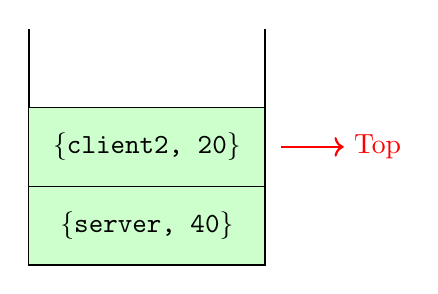
\begin{tikzpicture}
    % Draw stack container
    \draw[thick] (0,0) -- (0,3);  % left side
    \draw[thick] (3,0) -- (3,3);  % right side
    \draw[thick] (0,0) -- (3,0);  % bottom
    
    % Stack items
    \draw[fill=green!20] (0,0) rectangle (3,1) node[midway]{\texttt{\{server, 40\}}};
    \draw[fill=green!20] (0,1) rectangle (3,2) node[midway]{\texttt{\{client2, 20\}}};
 
    % Arrow and label (top of stack)
    \draw[->, thick, red] (3.2,1.5) -- (4,1.5) node[right]{Top};
\end{tikzpicture}
\caption{A stack with four entries.}
\label{fig:stack2}
\end{figure}

After that more messages might come into the mailbox of our monitor, since we
can have multiple client interactions, that is why it is crucial to have the
context association so that we always work within the correct causal context
when evaluating our formula by the monitor. An important note, is that between
the same causal chain, when there is an ordering in terms of actions, those will
always be followed, what we mean by this, is that the monitor will never see the
message \texttt{\{server, 40\}} before \texttt{\{client2, 20\}}, the question arises
when the system is dealing with multiple clients from different contexts.
\fi
\section{A Monitor On The Go}
\label{sec:waltz_monitor_example}

Finally, knowing everything up until this point, we can now present a fully developed example, from
specification to monitor generation and execution.

\subsection{Chat Room System}
\label{sub_sec:waltz_chatroom}

Consider the example introduced in \Cref{cha:background}, a chat system where
multiple clients can connect and post messages. To provide a more
\texttt{Erlang} oriented view of the system, it is essential to clearly define
the communication protocol, as this directly influences how properties should
be specified and monitored.

In this system, clients first establish a connection, then enter a chat room,
and finally post messages within that room. These interactions are illustrated
in \Cref{fig:connectserver}, \Cref{fig:enterroom}, and \Cref{fig:postmsg}.

\begin{figure}[ht]
\centering
\usetikzlibrary{arrows.meta, positioning, automata, shapes.geometric}
\scalebox{0.8}{%
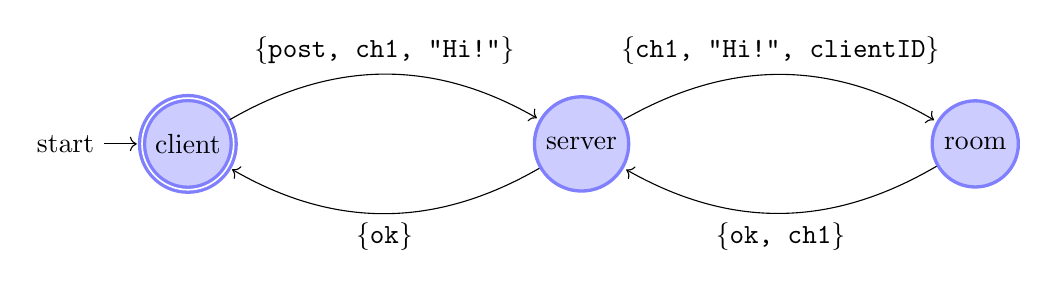
\begin{tikzpicture}[shorten >=1pt,node distance=5cm,on grid,
    every state/.style={draw=blue!50,very thick,fill=blue!20}]
  \tikzstyle{nodeB}=[circle,thick,draw=gray!75,fill=blue!20,minimum size=15mm]
  % States
  \node[nodeB, state, accepting, initial] (q1) {client};
  \node[nodeB, state] (q2) [right=of q1] {server};
  \node[nodeB, state] (q3) [right=of q2] {room};

  % Transitions
  \path[->] (q1) edge [bend left]  node[above] {\{\texttt{post, ch1, "Hi!"}\}} (q2);
  \path[->] (q2) edge [bend left]  node[below] {\{\texttt{ok}\}} (q1)
                 edge [bend left]  node[above] {\{\texttt{ch1, "Hi!", clientID}\}} (q3);
  \path[->] (q3) edge [bend left]  node[below] {\{\texttt{ok, ch1}\}} (q2);
         
\end{tikzpicture}
}
\caption{System behaviour for post action}
\label{fig:postmsg}
\end{figure}

\begin{figure}[ht]
\centering
\usetikzlibrary{arrows.meta, positioning, automata, shapes.geometric}
\scalebox{0.8}{%
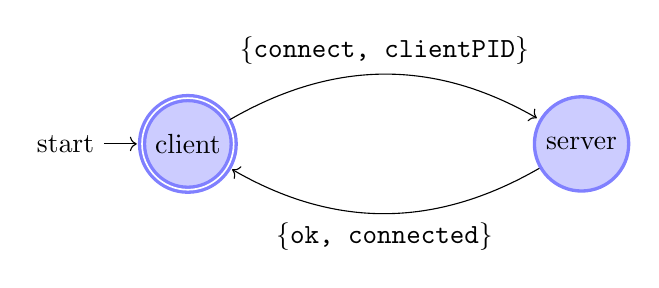
\begin{tikzpicture}[shorten >=1pt,node distance=5cm,on grid,
    every state/.style={draw=blue!50,very thick,fill=blue!20}]
  \tikzstyle{nodeB}=[circle,thick,draw=gray!75,fill=blue!20,minimum size=15mm]
  % States
  \node[nodeB, state, accepting, initial] (q1) {client};
  \node[nodeB, state] (q2) [right=of q1] {server};
   % Transitions
  \path[->] (q1) edge [bend left]  node[above] {\{\texttt{connect, clientPID}\}} (q2);
  \path[->] (q2) edge [bend left]  node[below] {\{\texttt{ok, connected}\}} (q1);

\end{tikzpicture}
}
\caption{System behaviour for login action}
\label{fig:connectserver}
\end{figure}

\begin{figure}[ht]
\centering
\usetikzlibrary{arrows.meta, positioning, automata, shapes.geometric}
\scalebox{0.8}{%
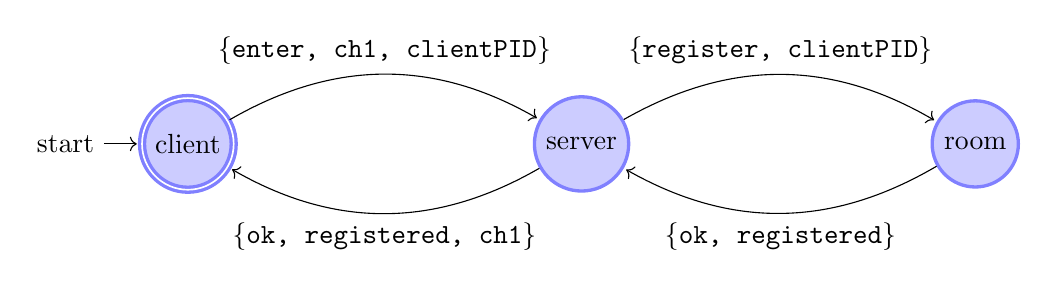
\begin{tikzpicture}[shorten >=1pt,node distance=5cm,on grid,
    every state/.style={draw=blue!50,very thick,fill=blue!20}]
  \tikzstyle{nodeB}=[circle,thick,draw=gray!75,fill=blue!20,minimum size=15mm]
  % States
  \node[nodeB, state, accepting, initial] (q1) {client};
  \node[nodeB, state] (q2) [right=of q1] {server};
  \node[nodeB, state] (q3) [right=of q2] {room};

  % Transitions
  \path[->] (q1) edge [bend left]  node[above] {\{\texttt{enter, ch1, clientPID}\}} (q2);
  \path[->] (q2) edge [bend left]  node[below] {\{\texttt{ok, registered, ch1}\}} (q1)
                 edge [bend left]  node[above] {\{\texttt{register, clientPID}\}} (q3);
  \path[->] (q3) edge [bend left]  node[below] {\{\texttt{ok, registered}\}} (q2);
         
\end{tikzpicture}
}
\caption{System behaviour for enter actions}
\label{fig:enterroom}
\end{figure}

This system exhibits a variety of interesting interactions that we can capture.
For instance, we might want to verify that once a client enters a chat room,
they can only post messages within that room and not elsewhere. In WALTZ, this
property can be formalized as follows:
\[
\varphi =
\Omega\left(
\begin{aligned} 
  &\quad\text{\texttt{send$_{\text{server} \rightarrow \text{client}}$}}\{ \text{\texttt{ok, registered, Room1}}\} : \top\ ; \\
  &\quad\quad\Omega(\text{\texttt{send$_{\text{client} \rightarrow \text{server}}$}}\{ \text{\texttt{post, Room2, Message}}\} : \text{\texttt{Room1 = Room2}})
\end{aligned}
\right)
\]

This property allows us to capture a part of each client’s interactions with
the system, verifying that all clients adhere to the expected rules:
specifically, no client can post a message in a channel where it is not
registered. Consider the following trace, where each sequence corresponds to a
different client communicating with the system:
\[
\begin{align*}
  \sigma_{\text{\texttt{c1}}} \;&=\; \{\text{\texttt{enter}}, \text{\texttt{ch1, ClientPID}}\} \ \{ \text{\texttt{ok, registered, ch1}}\} \ \{ \text{\texttt{post, ch1, Msg}}\}    \\
  \sigma_{\text{\texttt{c2}}} \;&=\; \{\text{\texttt{enter}}, \text{\texttt{ch2, ClientPID}}\} \ \{ \text{\texttt{ok, registered, ch2}}\} \ \{ \text{\texttt{post, ch1, Msg}}\} 
\end{align*}
\]

By examining the trace, we can see that the first client behaves correctly: it
enters a chat room and subsequently sends a message to that room. The issue
arises with the second client, which enters a different chat room and attempts
to send a message to a chat room it is not registered in, a clear violation of
the property we intend to monitor. It is important to remember that both
$\sigma_{\text{\texttt{c1}}}$ and $\sigma_{\text{\texttt{c2}}}$ are part of a
single trace $\sigma$ produced by the system. For simplicity and better
clarity, we can treat them as independent, isolated traces. In practice, the
monitor treats them as separate chains, verifying the property independently
for each context.

\iffalse
By looking at the trace, we can see that the first client is behaving
correctly, he enters a chat room, and after that send a message to it. The
problem is with the second client, that enters another chat room, and tries to
send a message to one that he is not registered, that is a clear violation of
the property that we want to check. Remember that, both
$\sigma_{\text{\texttt{c1}}}$ and $\sigma_{\text{\texttt{c2}}}$, are part of a
unique trace $\sigma$ being produced by the system, but in order to simplify
things for understanding we can think of them as isolated traces, and that is
what will happen in practice. The monitor responsible for verifying the
property will check these traces separately, guaranteeing that it verifies the
property per each context (each isolated chain).
\fi
\begin{erlang}[caption={\texttt{main\_monitor.erl}}, label={lst:monitorchatmain}]
monitor_loop(ContextMap) ->
  receive
    {Src, Dst, Msg, Context} ->
      case maps:get(Context, ContextMap, undefined) of
        undefined ->
          main_loop(Src, Dst, Msg, Context, ContextMap);
        PID ->
          PID ! {Src, Dst, Msg, Context},
          monitor_loop(ContextMap)
  end 
end.

main_loop(Src, Dst, Msg, Context, ContextMap) ->
  case {Src, Dst, Msg} of
    {server, client, {ok, registered, Room1}} ->
        if true ->
          Environment = #{room1 => Room1},
          SubPID = spawn(sub_monitor, [Environment, Context, self()]),
          NewContextMap = ContextMap#{Context => SubPID},
          monitor_loop(NewContextMap),
          ok
        ; true ->
          io:format("(*@$\text{\ding{56}}$@*)")
        end;
end.
\end{erlang}

The main monitoring loop that coordinates the verification process is shown in
Listing \ref{lst:monitorchatmain}. Here, the \texttt{main\_monitor.erl} process receives
all messages from the system, identifies or creates the appropriate sub-monitor
for the given context, and forwards messages to it. Each new client connection
triggers the creation of a sub-monitor, responsible for tracking that specific
client’s interactions.

Once a sub-monitor is spawned, it is responsible for evaluating all subsequent
messages in its assigned context. Listing \ref{lst:monitorchatsub} shows the
structure of a sub-monitor in \texttt{sub\_monitor.erl}. This process continuously
receives messages from the client, checks whether the client is posting to the
registered room, and either loops to process further messages or reports a
violation back to the main monitor. In our example, the second client
attempting to post in an unregistered room would trigger the sub-monitor to
notify the main monitor of the property violation.

\begin{erlang}[caption={\texttt{sub\_monitor.erl}}, label={lst:monitorchatsub}]
sub_monitor(Environment, Context, ParentPID) ->
  receive
    {client, server, Msg, Context} ->
      case Msg of
        {post, Room2, _} ->
          if maps:get(room1, Environment) == Room2 ->
            sub_monitor(Environment, Context, ParentPID)
          ; true ->
            ParentPID ! {context_completed, Context, (*@$\text{\ding{56}}$@*)}
          end;
        _ ->
          sub_monitor(Environment, Context, ParentPID)
      end;
  end.
\end{erlang}

\iffalse
\begin{erlang}[caption={\texttt{monitor.erl}}, label={lst:monitorchat}]
% main_monitor.erl
monitor_loop(ContextMap) ->
  receive
    {Src, Dst, Msg, Context} ->
      case maps:get(Context, ContextMap, undefined) of
        undefined ->
          main_loop(Src, Dst, Msg, Context, ContextMap);
        PID ->
          PID ! {Src, Dst, Msg, Context},
          monitor_loop(ContextMap)
  end 
end.

main_loop(Src, Dst, Msg, Context, ContextMap) ->
  case {Src, Dst, Msg} of
    {server, client, {ok, registered, Channel1}} ->
        if true ->
          Environment = #{channel1 => Channel1},
          SubPID = spawn(sub_monitor, [Environment, Context, self()]),
          NewContextMap = ContextMap#{Context => SubPID},
          monitor_loop(NewContextMap),
          ok
        ; true ->
          io:format("(*@$\text{\ding{56}}$@*)")
        end;
end.
%sub_monitor.erl
sub_monitor(Environment, Context, ParentPID) ->
  receive
    {client, server, Msg, Context} ->
      case Msg of
        {post, Channel2, _} ->
          if maps:get(channel1, Environment) == Channel2 ->
            sub_monitor(Environment, Context, ParentPID)
          ; true ->
            ParentPID ! {context_completed, Context, (*@$\text{\ding{56}}$@*)}
          end;
        _ ->
          sub_monitor(Environment, Context, ParentPID)
      end;
  end.
\end{erlang}
\fi

This monitor exemplifies the strengths of WALTZ, including hierarchical context
management, correlation of messages across multiple interactions, and the
evaluation of properties over all contexts present in the system. The use of
nested modal operators necessitates more than a single monitor, as relying on
just one would result in the monitor being indefinitely occupied with a single
context. By spawning separate processes for sub-monitors, we enable concurrent
monitoring of multiple contexts, while the main oracle orchestrates the routing
of messages to their corresponding child monitors.

When examining the trace of the second client, $\sigma_{\text{\texttt{c2}}}$,
the property violation becomes apparent. The sub-monitor evaluates the
condition \texttt{Room1 == Room2}, which fails because the client
attempts to post to a chat room that is different from the one it entered. This
violation of property $\varphi$ is detected at runtime, demonstrating how the
WALTZ-generated monitor successfully enforces correctness across concurrent
client interactions.

\iffalse
\section{Optimizations}
\label{sec:waltz_optimizations}

In this section, we will explain what possible optimizations we can performs in order to
make our monitors more concurrent friendly. Introducing the main oracle management
of contexts, spawning multiple monitors and the destruction of them when possible to
avoid unnecessary overhead.

One of the optimizations that we could perform is the simplification of properties
with the following structure: $\Theta(\Theta(\alpha : \delta))$, because we can then
state that they are essentially the same as checking for $\Theta(\alpha : \delta)$.

Then another optimization, is in order to allow multiple verifications per monitor, in
properties like $\Theta(\alpha : \delta)$, we might spawn multiple monitors, an kill them
on the go, allowing for more concurrency on the monitor side. There is even a possible
optimization where we even ignore the messages of a dead chain, instead of consuming them. 

If time is our ally, we will do these and refer to them in the thesis, for now
let's leave this like that and focus on the next chapter.
\fi
\section{Monitorability of WALTZ}
\label{sec:waltz_monitorability}
Like any specification language, WALTZ is not immune to the issue of
non-monitorability. It is possible to restrict the language to a monitorable
fragment, but doing so comes at the cost of expressiveness. For instance,
consider the property $\varphi_1 =$ "For every client, at least one of his
requests is a positive number". Due to the inherently infinite nature of
runtime traces, this property is non-monitorable, as discussed
in~\cite{pnueli2006psl}. Similarly, a property such as $\varphi_2 =$ "At least
for one client, all his messages have a positive number" is also
non-monitorable. In this case, we depend on an event occurring infinitely often
to guarantee satisfaction for at least one client, which, again, prevents
runtime monitors from ever yielding a conclusive verdict.

There are properties that can be expressed in WALTZ and are meaningful from a
specification perspective, but in practice, they are non-monitorable. This is
because the monitor would never be able to reach a conclusive verdict,
resulting in a continuously running process that consumes system resources,
adds overhead, and ultimately provides no useful feedback.
While there is ongoing research aimed at expanding the set of monitorable
properties, and attempts to transform certain non-monitorable properties into
monitorable ones~\cite{ferrando2025towards, ferrando2025towards}, some properties remain inherently
non-monitorable unless additional assumptions or modifications are made.

For example, consider the property $\varphi_1 = \Omega(\alpha_1 : \delta_1 \ ;
\ \Theta(\alpha_2 : \delta_2))$ whose context structure tree is illustrated in
\Cref{fig:non_monone}. As we will see, the nesting between the $\Omega$ and
$\Theta$ operators makes it impossible for a runtime monitor to ever produce a
conclusive verdict in this scenario. 

\begin{figure}[ht]
\centering
\usetikzlibrary{arrows.meta, positioning, automata, shapes.geometric}
\scalebox{1}{%
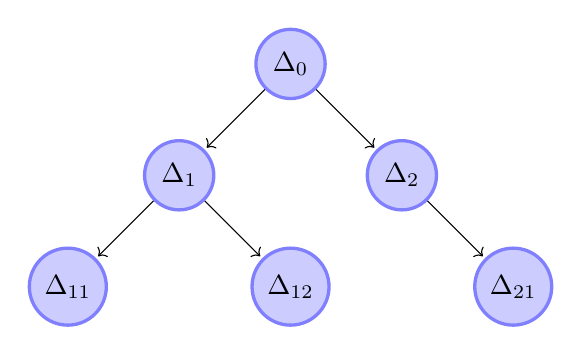
\begin{tikzpicture}[shorten >=1pt,node distance=2cm,on grid,
    every state/.style={draw=blue!50,very thick,fill=blue!20}]
  % Define square nodes instead of circles
  \tikzstyle{nodeG}=[rectangle,thick,draw=gray!75,fill=green!20,minimum size=10mm]
  \tikzstyle{nodeR}=[rectangle,thick,draw=gray!75,fill=red!20,minimum size=10mm]
  \tikzstyle{nodeB}=[rectangle,thick,draw=gray!75,fill=blue!20,minimum size=10mm]
  \tikzstyle{nodeI}=[state, rectangle,thick,draw=gray!75,fill=blue!20,minimum size=10mm]
  \tikzstyle{nodeGray}=[rectangle,thick,draw=gray!75,fill=gray!30,minimum size=10mm]
 
  \node[nodeGray, state]          (q_000)              {$\Delta_0$};
  \node[nodeGray, state]          (q_111) [below right=of q_000] {$\Delta_2$};
  \node[nodeGray, state]          (q_222) [below left=of q_000] {$\Delta_1$}; 
  \node[nodeB, state]             (q_333) [below left= of q_222] {$\Delta_{11}$};
  \node[nodeB, state]             (q_555) [below right= of q_222] {$\Delta_{12}$};
  \node[nodeB, state]             (q_666) [below right = of q_111] {$\Delta_{21}$};
 
  \path[->] (q_000) edge node [above right]  {} (q_111);
  \path[->] (q_000) edge node [above left] {} (q_222);
  \path[->] (q_222) edge node [above right] {} (q_555);
  \path[->] (q_222) edge node [above left] {} (q_333);
  \path[->] (q_111) edge node [above right] {} (q_666);
\end{tikzpicture}
}
\caption{Monitor organization for $\varphi_1$}
\label{fig:non_monone}
\end{figure}

Examining the structure depicted in \Cref{fig:non_monone}, we can describe the
waiting behaviour of each monitor within the hierarchy of contexts. In this
setup, $\Delta_0$, which is the parent of all contexts monitored by the
$\Omega$ operator, waits for a property violation in order to produce a
conclusive verdict. Meanwhile, the child contexts, such as those under
$\Delta_1$ and $\Delta_2$, are monitored by the $\Theta$ operator. These
sub-monitors are waiting for a satisfaction to produce a verdict, as this is
the fundamental behaviour of $\Theta$. The problem arises because $\Theta$
monitors can never output a negative verdict, they can only yield a positive
verdict or remain inconclusive.

As a result, $\Delta_0$ will never receive the violation signal it needs to
reach a conclusive verdict. Instead, it is left waiting indefinitely while its
children either satisfy the property or remain inconclusive. This interplay of
waiting and verdict-passing is clearly illustrated in \Cref{fig:nonmontree1},
highlighting why this property is inherently non-monitorable at runtime.

\begin{figure}[ht]
\centering
\usetikzlibrary{arrows.meta, positioning, automata, shapes.geometric}
\scalebox{1}{%
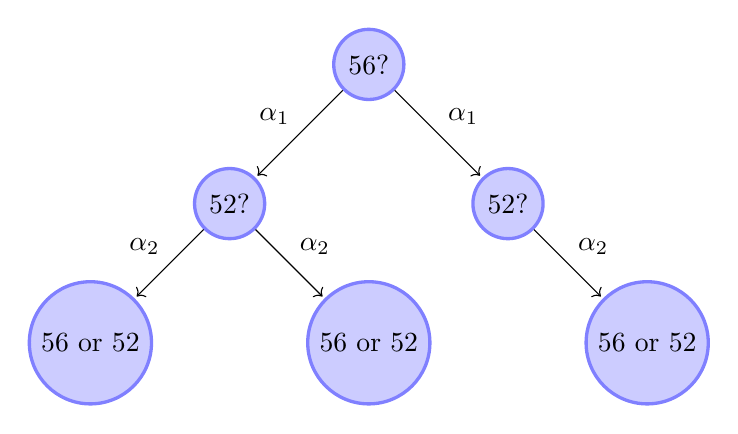
\begin{tikzpicture}[shorten >=1pt,node distance=2.5cm,on grid,
    every state/.style={draw=blue!50,very thick,fill=blue!20}]
  % Define square nodes instead of circles
  \tikzstyle{nodeG}=[rectangle,thick,draw=gray!75,fill=green!20,minimum size=10mm]
  \tikzstyle{nodeR}=[rectangle,thick,draw=gray!75,fill=red!20,minimum size=10mm]
  \tikzstyle{nodeB}=[rectangle,thick,draw=gray!75,fill=blue!20,minimum size=10mm]
  \tikzstyle{nodeI}=[state, rectangle,thick,draw=gray!75,fill=blue!20,minimum size=10mm]
  \tikzstyle{nodeGray}=[rectangle,thick,draw=gray!75,fill=gray!30,minimum size=10mm]
 
  \node[nodeGray, state]          (q_000)              {\ding{56}?};
  \node[nodeGray, state]          (q_111) [below right=of q_000] {\ding{52}?};
  \node[nodeGray, state]          (q_222) [below left=of q_000] {\ding{52}?}; 
  \node[nodeB, state]             (q_333) [below left= of q_222] {\ding{56} or \ding{52}};
  \node[nodeB, state]             (q_555) [below right= of q_222] {\ding{56} or \ding{52}};
  \node[nodeB, state]             (q_666) [below right = of q_111] {\ding{56} or \ding{52}};
 
  \path[->] (q_000) edge node [above right]  {$\alpha_1$} (q_111);
  \path[->] (q_000) edge node [above left] {$\alpha_1$} (q_222);
  \path[->] (q_222) edge node [above right] {$\alpha_2$} (q_555);
  \path[->] (q_222) edge node [above left] {$\alpha_2$} (q_333);
  \path[->] (q_111) edge node [above right] {$\alpha_2$} (q_666);
\end{tikzpicture}
}
\caption{Non-monitorable structure for $\varphi_1$}
\label{fig:nonmontree1}
\end{figure}

A related, yet distinct, challenge arises when monitoring for properties that
require at least one instance in the domain to satisfy a given condition. In
this case, the monitor’s ability to reach a verdict depends on an event
occurring at some point in the future, potentially indefinitely, which we
cannot guarantee at runtime. Even if a violation occurs, which might allow a
partial conclusion, the monitor must continue observing, since we are
specifically interested in finding at least one context that satisfies the
property. This inherent uncertainty renders such properties non-monitorable. An
example of this scenario is the property $\varphi_2 = \Theta(\alpha_1 :
\delta_1 \ ; \ \Omega(\alpha_2 : \delta_2))$ whose monitor structure is
illustrated in \Cref{fig:nonmontree2}. 

\begin{figure}[ht]
\centering
\usetikzlibrary{arrows.meta, positioning, automata, shapes.geometric}
\scalebox{1}{%
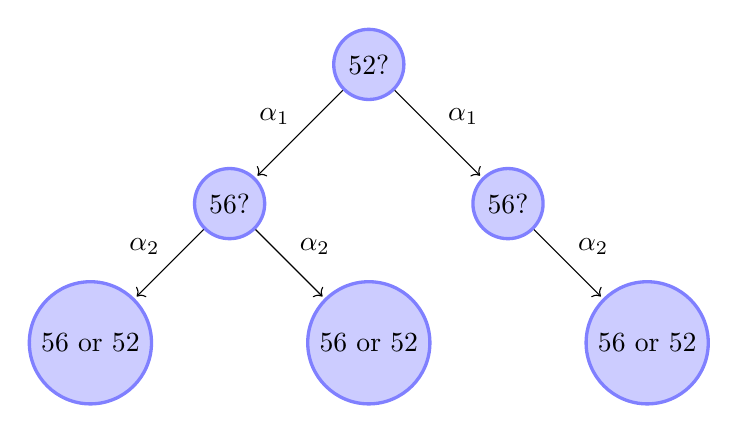
\begin{tikzpicture}[shorten >=1pt,node distance=2.5cm,on grid,
    every state/.style={draw=blue!50,very thick,fill=blue!20}]
  % Define square nodes instead of circles
  \tikzstyle{nodeG}=[rectangle,thick,draw=gray!75,fill=green!20,minimum size=10mm]
  \tikzstyle{nodeR}=[rectangle,thick,draw=gray!75,fill=red!20,minimum size=10mm]
  \tikzstyle{nodeB}=[rectangle,thick,draw=gray!75,fill=blue!20,minimum size=10mm]
  \tikzstyle{nodeI}=[state, rectangle,thick,draw=gray!75,fill=blue!20,minimum size=10mm]
  \tikzstyle{nodeGray}=[rectangle,thick,draw=gray!75,fill=gray!30,minimum size=10mm]
 
  \node[nodeGray, state]          (q_000)              {\ding{52}?};
  \node[nodeGray, state]          (q_111) [below right=of q_000] {\ding{56}?};
  \node[nodeGray, state]          (q_222) [below left=of q_000] {\ding{56}?}; 
  \node[nodeB, state]             (q_333) [below left= of q_222] {\ding{56} or \ding{52}};
  \node[nodeB, state]             (q_555) [below right= of q_222] {\ding{56} or \ding{52}};
  \node[nodeB, state]             (q_666) [below right = of q_111] {\ding{56} or \ding{52}};
 
  \path[->] (q_000) edge node [above right]  {$\alpha_1$} (q_111);
  \path[->] (q_000) edge node [above left] {$\alpha_1$} (q_222);
  \path[->] (q_222) edge node [above right] {$\alpha_2$} (q_555);
  \path[->] (q_222) edge node [above left] {$\alpha_2$} (q_333);
  \path[->] (q_111) edge node [above right] {$\alpha_2$} (q_666);
\end{tikzpicture}
}
\caption{Non-monitorable structure for $\varphi_2$}
\label{fig:nonmontree2}
\end{figure}

As illustrated in \Cref{fig:nonmontree2}, the main monitor is waiting to detect
a satisfaction, but none of its child monitors can provide this information. At
most, they are able to detect violations, and under normal execution, they will
continue emitting inconclusive verdicts (denoted by \texttt{?}) indefinitely.
As a result, the main monitor is never able to determine conclusively whether
the property has been satisfied, leaving the system in a state of perpetual
uncertainty.

To illustrate when a property is fully monitorable, we can consider the example
of the property $\varphi_3 = \Omega(\alpha : \delta)$. The monitor structure
for this property is shown in \Cref{fig:montree1}.

\begin{figure}[ht]
\centering
\usetikzlibrary{arrows.meta, positioning, automata, shapes.geometric}
\scalebox{1}{%
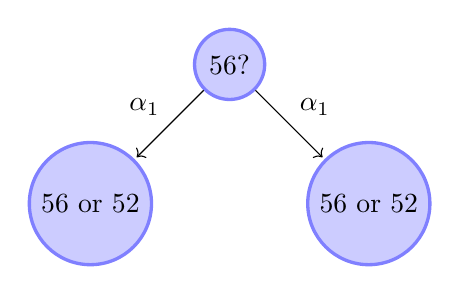
\begin{tikzpicture}[shorten >=1pt,node distance=2.5cm,on grid,
    every state/.style={draw=blue!50,very thick,fill=blue!20}]
  % Define square nodes instead of circles
  \tikzstyle{nodeG}=[rectangle,thick,draw=gray!75,fill=green!20,minimum size=10mm]
  \tikzstyle{nodeR}=[rectangle,thick,draw=gray!75,fill=red!20,minimum size=10mm]
  \tikzstyle{nodeB}=[rectangle,thick,draw=gray!75,fill=blue!20,minimum size=10mm]
  \tikzstyle{nodeI}=[state, rectangle,thick,draw=gray!75,fill=blue!20,minimum size=10mm]
  \tikzstyle{nodeGray}=[rectangle,thick,draw=gray!75,fill=gray!30,minimum size=10mm]
 
  \node[nodeGray, state]          (q_000)              {\ding{56}?};
  \node[nodeGray, state]          (q_111) [below right=of q_000] {\ding{56} or \ding{52}};
  \node[nodeGray, state]          (q_222) [below left=of q_000] {\ding{56} or \ding{52}}; 
 
  \path[->] (q_000) edge node [above right]  {$\alpha_1$} (q_111);
  \path[->] (q_000) edge node [above left] {$\alpha_1$} (q_222);

\end{tikzpicture}
}
\caption{Monitorable property}
\label{fig:montree1}
\end{figure}

As we can see from the figure, the oracle monitor is waiting for a potential
violation. Each sub-monitor associated with a specific context either detects a
violation or observes satisfaction. Because the property requires that all
contexts satisfy the condition, a violation detected in any single leaf context
is sufficient for the oracle to yield a conclusive verdict. This demonstrates
how, in this scenario, the monitor can effectively reach a verdict,
highlighting the monitorable nature of $\varphi_3$.

The issue of non-monitorability arises primarily because we are dealing with
potentially infinite traces. If the trace were finite, however, all of these
properties would become monitorable, since we could examine the trace in its
entirety and produce a conclusive verdict. This approach, however, requires
offline monitoring, which cannot alert the system to violations in real time.
Later in this document, we outline concrete strategies, both in a general sense
and specifically for actor-based systems, that enable monitoring of properties
that would otherwise be non-monitorable at runtime.


